\documentclass{article}
\usepackage[utf8]{inputenc}
\usepackage{algorithm}
\usepackage{algorithmic}
\usepackage{amsfonts}
\usepackage{graphicx}
\usepackage{listings}
\usepackage{xcolor}
\usepackage{amsmath}
\usepackage{amsthm,amssymb}
\theoremstyle{definition}
\theoremstyle{theorem}
\usepackage{geometry}
\usepackage[magyar]{babel}
\geometry{a4paper,outer=25mm,inner=35mm,top=25mm,bottom=25mm}
\linespread{1.5}
\frenchspacing
\newtheorem{definition}{Definíció}
\newtheorem{theorem}{Tétel}

\newtheorem{example}{Példa}
\renewcommand{\qedsymbol}{\rule{0.7em}{0.7em}}
\title{Szakdolgozat}
\author{Szabó Bence Dániel }
\date{Date}

\definecolor{codegreen}{rgb}{0,0.6,0}
\definecolor{codegray}{rgb}{0.5,0.5,0.5}
\definecolor{codepurple}{rgb}{0.58,0,0.82}
\definecolor{backcolour}{rgb}{0.95,0.95,0.92}

\lstdefinestyle{mystyle}{
    backgroundcolor=\color{backcolour},
    commentstyle=\color{codegreen},
    keywordstyle=\color{magenta},
    numberstyle=\tiny\color{codegray},
    stringstyle=\color{codepurple},
    basicstyle=\ttfamily\footnotesize,
    breakatwhitespace=false,
    breaklines=true,
    captionpos=b,
    keepspaces=true,
    numbers=left,
    numbersep=5pt,
    showspaces=false,
    showstringspaces=false,
    showtabs=false,
    tabsize=2
}
\lstset{style=mystyle}
\begin{document}

\begin{center}
\fontsize{40pt}{12pt}\selectfont

    DIFFERENCIÁLEGYENLETEK NUMERIKUS MEGKÖZELÍTÉSE A KÖZGAZDASÁGBAN\\
    \bigskip
    Szabó Bence Dániel \\
    \bigskip
    2022
\end{center}

\pagebreak

\begin{center}
\fontsize{40pt}{12pt}\selectfont
    Budapesti Corvinus Egyetem \\
    \bigskip
    Készítette: Szabó Bence Dániel \\
    \bigskip
    Konzulens: Dr. Kánnai Zoltán\\
    \bigskip
    2022
\end{center}
\pagebreak
\tableofcontents
\pagebreak
\section{Bevezetés}
A szakdolgozatomat szerettem volna egybekötni a programozással, ezen belül a Python nyelvvel és annak különböző részeivel, illetve a differenciálegyenletek numerikus megoldásaival. Ez azonban meglepően sok számomra eddig ismeretlen területet mutatott meg, ilyen volt például a dekorátorok használata, az ábra készítő csomagok működési elve, illetve az oszlopműveletek hatékonysága, beleértve a kapcsolatot az alacsonyabb szintű programozási nyelvekkel. Ezután jobban megértettem, hogy mit is jelent egy programozási nyelv és milyen hasonlóságok és eltérések lehetnek a különböző nyelvek között. A szakirodalom olvasása közben képet kaptam arról, hogy amikor a modellezésben előkerülnek a differenciálegyenletek, akkor a különböző tudományágak képviselői milyen megközelítésekkel szoktak élni a kutatásuk során, és ennek milyen következményei lehetnek a cikkekre ,amiket írtak.

Ahol programozható problémával találkoztam, ott törekedtem arra, hogy csatoljak hozzá egy általam megírt kódot, követve a Python nyelv hivatalos útmutatóit. Ehhez segítségül is vettem a black csomagot, ami átrendezte a kódom, ha az nem felelt meg valamilyen formázási útmutatónak. Természetesen ez funkcionalitást semmilyen mértékben nem érintett, csak az olvashatóságon javított nagy mértékben. Mivel sokat fordul elő kód a szakdolgozatban, így próbáltam egy tömör Python bevezetőt is elkészíteni, mert úgy gondoltam, hogy így lehet teljes a dolgozat. Célom volt,  hogy amit csak lehet, öntsek matematikai formalizmusba.  A differenciálegyenletek elmélete nem egyszerű témakör a matematikán belül és a szakdolgozatnak nem is volt célja, hogy teljesen matematikai szempontból tárgyaljam a kérdést, mert ahhoz ez túl nehéz problémakör és meghaladná  a szakdolgozat fizikai kereteit. A numerikus analízis, aminek az eszköztárát vettem segítségül úgyszintén egy nehéz és kiterjedt ága a matematikának és innen is csak érintőlegesen használtam módszereket.

A lehető legnagyobb figyelmet próbáltam szentelni annak a takarékossági szempontnak, hogy a kód legyen a tőlem telhető leghatékonyabb. Miközben erre figyeltem, szépen összeállt egy kép előttem, nevesen az, hogy az alapvető közgazdasági tételek ebben a világban is érvényesülnek, mégpedig az, hogy akkor tudunk a legtöbbet spórolni, ha a költségeinket a lehető legkisebb értékre redukáljuk. Ez mindig is szempont volt, amióta léteznek számítógépek, mert egy nem optimálisan megírt algoritmus sok ideig futhat, ezzel pedig több áramot fogyasztunk, ami például egy nagy adathalmazra nézve sok pénzt jelenthet, ha megnézzük a számítási kapacitások árát, főleg ha gyakoriak a feladatok, amire a kódot megírtuk.

Mivel én is sokat tanultam a szakdolgozat írása közben, olyan módon próbáltam felépíteni az egészet, ha valaki járatlan a témában és kezébe veszi a dolgozatomat, akkor is könnyen megértse annak mondandóját. Egyfajta összefoglaló volt a célom, mintha csak demonstrátorként készítettem volna elő egy kurzusszemeszter anyagát.
\section{Szakirodalmi áttekintő}
A differenciálegyenletek használata nagyon sok területen megjelenik az alkalmazott matematikán belül. A közgazdasági modellek körében számottevő módon használják a dinamikai rendszerek eszköztárát. Itt alapvetően azt vizsgálják a kutatók, hogy az idő változásával hogyan és miképp változik meg egy-egy rendszer és annak a változói. Amint feltudtuk írni az egyenleteket akkor vizsgálhatjuk a rendszer stabilitáselméleti 'diagnosztikáit', amit majd látjuk a következő részekben, hogy a sajátértékek vizsgálatából von le következtetéseket, ezt felhasználva tudunk valamit mondani a rendszer  időbeli fejlődéséről.\newline
A dinamikai rendszerek másik érdekes ága a káoszelmélet. Ez az irány olyan nemlineáris dinamikai rendszereket vizsgál, amelyek ugyan determinisztikus modellek, mégis nagyon nehéz az előrejelzésük még rövid időtávra is nézve. Guégan \cite{GUEGAN200989} cikkében ad egy általánosabb összefoglalót arra, hogy a különböző problémákra milyen modelleket érdemes használni, illetve összehasonlítja, hogy a tudományágak képviselői milyen módon építenek dinamikai rendszereket.
Azt mondja, hogy egy közgazdász próbálja megérteni a vizsgált helyzetet és leírni, egy fizikus pedig az adatokból az univerzum törvényeit próbálja megérteni. A káoszelmélet következtetéseit pedig a bifurkációk vizsgálatával nézik. Lorenz \cite{Lorenz1994} nemlineáris Keynesi modellt épített. Megemlíti, hogy a legtöbb mikró- és makróökonómiai modell egyensúlyt keres amellett, hogy felteszik az egyéni racionalitást. Az egyéneket leíró egyenleteket pedig lineáris függvényként definiálja, felteszi a reprezentatív egyént és innen az aggregált szinten is az összefüggések lineárisak lesznek. Szerinte azonban egy stabil gazdasághoz nem feltétlenül kell egyensúly nemlineáris esetben. Azért sem lesz elég a szerző szerint, mert ha megkerestük a modell fixpontját, kiazámoltuk a stabilitási mutatókat az nem lesz elég, mert a sok paraméter miatt érzékeny marad az egész rendszer a többi változó sokkolására. Természetesen a valóság megkövetel bizonyos esetekben magasabb dimenziójú modelleket, azonban ez magával hoz egy következő problémát, mégpedig azt, hogy a kényszerűen megtett pótlólagos feltevések mögött húzódik-e meg bárminemű közgazdasági relevancia. Ha erre nem bírunk pozitív válasszal, akkor vizsgálatunk könnyen elmehet tisztán matematikai irányba. Azonban a szerző szerint ezek az állítások úgyszintén igazak magára a nemlinearitásra is. Ezáltal azt mondja, hogy csak akkor ragadjanak meg nemlineáris mintaillesztést, ha arra találnak közgazdasági relevanciát. Végezetül arról is beszél Lorenz, hogy mindezek igazak a kaotikus modellezésre is. Azaz amennyiben az empirikus adatsor nem tartalmaz olyan motívumokat amelyek arra utalnak, hogy jól megragadható a folyamat bizonyos kaotikus egyenletekkel, akkor nem érdemes belevágni.\newline
Az egyik legrégebbi dinamikus modellt \cite{Ezekiel} az 1930-as években alkotta meg Ezekiel. Itt az volt a forradalmi ötlet, hogy eltolta a kereslet és a kínálat közötti kapcsolatot 1 időegységgel olyan piacokon, ahol romlandó termékekkel foglalkoznak. Ez azt jelenti, hogy a keresletre a válasz az előző időszakban megtermelt mennyiség lesz a válasz. Matematikailag felírva ezt a következőképpen formalizálhatjuk :
\begin{equation*}
    D(t) = S(t-1)
\end{equation*}
Ezzel az összefüggéssel kapcsolta össze az idő múlását Ezekiel a rendszerrel. Az így kapott eredményt pedig pókháló modellnek nevezte el, mivel ha összekötötte a kétdimenziós ábrán a keresletet és a kínálatot, pókhálószerű ábra rajzolódott ki. A pókhláló modell ezután több szerzőt is megihletett és mélyebb matematikai összefüggéseket kezdtek el kutatni a pókháló séma mentén. Egyik ilyen kutatási eredmény \cite{HOMMES1994315} az, ahol feloldották a kereslet és a kínálat lineáris felépítését és adaptív várakozásokat építettek bele a modellbe, amellett, hogy mind a kereslet és mind a kínálat monoton leképezések voltak. Alapvetően ez is egy kaotikus megközelítést alkalmaz és a fő eredménye a cikknek az, hogy a modell ugyan nem működik valós adatokra, viszont a matematikai értelemben vett káosz egyszerű feltételek mellett is ki tud alakulni, ráadásul ezeknek a feltételezéseknek még közgazdasági relevanciája is van. Több kutató vizsgálta, hogy mi történik akkor, amikor feloldják akár az egyik függvény monotonitását \cite{Artstein1983} \cite{JENSEN1984235} \cite{LICHTENBERG1989225} és arra az eredményre jutottak, hogy ezesetben kialakul az árban egy kaotikus fluktuáció. Végezetül a pókháló modellcsaládhoz említsük meg \cite{DIECI20092011} munkáját. A szerzőpáros úgy módosította a pókháló modellt, hogy megengedett interakciót egy 2 termékes rendszerben. Ez azt jelentette, hogy a termelő tudta hangolni a kibocsátását az egyik és a másik termékből. Példaként hozták egy farmer esetét, aki visszaveheti a rizstermelés volumenét a búza javára. Ez a lehetőség a rendszert a nemlinearitás miatt elég hamar kaotikussá teheti, ami a különböző paraméterekre való érzékenység révén meglehetősen megnehezíti az egyszerű következtetések levonását. Ez amiatt történik, mert ha az egyik termék drágább lesz, akkor megnő az azt termelő egyének száma, ez pedig kibillenti a másik termék kínálatát a másik irányba. A szerzőpáros szerint tanulságos lehetnek az eredmények a kormányzati szervek számára, mert ezzel megtudják ragadni, hogy egy-egy piaci beavatkozás az állam részéről milyen hatásokat tudhat generálni a többi szektorban. Korrekt módon beszél a kutatás gyenge pontjairól és annak továbbfejleszthetőségéről, nevesen arról például, hogy nem elég általános a matematikai absztrakciója a modellnek, illetve nincs beépítve termékgyártás átváltási költség sem, ezen felül pedig érdemes megvizsgálni, hogy mely közgazdasági feltevések okoznak kaotikus viselkedést.
\newline A követekző cikkben \cite{Tacchella} egy olyan dinamikai rendszert építettek, amely a vizsgált országok GDP változását (akár növekedését, akár csökkenésést) volt hivatott előrejelezni. A szerzők megemlítik, hogy a GDP előrejelzés egy nehéz és komplex feladat, mivel rengeteg változóból épül fel ez a negyedévente / évente megszülető adat, ezen felül sok utólagos korrigálásban részesülnek az adatok, amelyek nem jól modellezhetőek, mert szubjektívan készítik el őket. Az eredményeiket jelentősnek írták le, mivel 25 százalék feletti eredménnyel jelezték előre a változást a hivatalos IMF statisztikákhoz képest, ezenfelül az IMF hibái és ő hibáik között alacsony volt a korreláció, ami azt jelenti, hogy az eltéréseik között nem volt érdemi információs átfedés, így új összefüggésekre tudtak rámutatni. A szerzők kiemelnek egy fontos tényezőt a közgazdasági modellezéssel kapcsolatban, hogy maga a közgazdaságtan, az elméleti modellezés és az előrejelzés tudományágak nincsenek szervesen összekapcsolva. A közgazdasági modellépítés azon alapszik, hogy vesznek a kutatók egy leegyszerűsített világot, majd egy változó hatását próbálják megérteni. Ezzel a megközelítéssel szemben a szerzők úgy álltak a problémához, hogy fizikusi szemmel kiváncsiak egy dinamikai rendszer időbeli fejlődésére olyan korlátozással, hogy egyedül csakis a múltbéli adatokra támaszkodhat. Ez azt jelenti, hogy az információ a historikus adatok és az adatpontok közötti időből nyerhető ki, nem tesznek feltevéseket mögé, tiszta lappal indulnak. A cikk bemutat egy nagyon érdekes módszert, angolul a 'method of analogues' módszert, ami azon az elgondoláson alapul, hogy amikor előre szeretnénk jelezni, de nincs információnk a rendszer épp aktuális állapotáról, akkor megnézzük, hogy a meglévő állapotok közül a jelenlegi ponthoz legközelebb álló helyzete miképp fejlődőtt egyik pillanatból a másikba, majd ezzel a tudással a kezünkben haladunk tovább. Az elemzés során felhasználták a \textit{fittség-komplexitás} (fitness-complexity) algoritmust, ami egy iteratív képlet és kapcsolatban áll a dinamikai rendszer megközelítéssel. A haszna az előrejelzésekben jelenik meg. Gyakorlatilag egy inputot vár el, mégpedig egy olyan mátrixot, amiben reprezentálják a gazdaságok export felépítését. Ez azt jelenti, hogy a sorok az országokat jelentik, az oszlopok a különböző termékeket. Ha az adott ország adott termékből kompetitíven képes exportálni, akkor 1-es értéket kap, ha nem akkor 0-t. Egyik előnye, hogy nem függ a kezdeti értékektől, de részletesebben megtalálhatjuk a jellemzőit a többi cikkben. Az algoritmust a következő féle képpen írták fel a cikk szerzői:
\begin{equation*}
    \begin{cases}
    \widetilde{F}_{c}^{(N + 1)} = \sum_{p} M_{cp} Q_{p}^{(N)} \\
    \widetilde{Q}_{p}^{(N+1)} = (\sum_{c} \frac{M_{cp}}{F_c^N})^{-1} \\

    \end{cases}
\end{equation*}
Itt M jelöli a fent említett bináris mátrixot, a c index jelöli az országot (country),a p index pedig az adott terméket (product). A nem hullámmal jelölt mennyiségek képletei is ismertek. Ezek gyakorlatilag mindig egy normalizált értéket adnak a következő iterációs lépéshez.
\begin{equation*}
    \begin{cases}
    F_c^{(N)} = \frac{\widetilde{F}_{c}^{(N)}}{<\widetilde{F}>_c} \\
    Q_p^{(N)} = \frac{\widetilde{Q}_{c}^{(N)}}{<\widetilde{Q}>_p}
    \end{cases}
\end{equation*}


\section{Python nyelv}

A Python egy nyílt forráskódú, magas szintű programozási nyelv egy könnyen elsajátítható szintaxissal. Azért erre a nyelvre esett
a választásom, mert sok csomag elérhető hozzá, nagyon jól dokumentált, nem kell típusokat használni benne az
esetek többségében. Nagyon elterjedt nyelvről beszélünk, ami rengeteg szakterületén jelen van a programozói világban. Emiatt pedig könnyen fórumozható, illetve karban vannak tartva a csomagok a nagy felhasználói létszám miatt. Alapvetően a nyelv arra épít, hogy kevés funkcionalitás érhető el benne, és ha szükségünk van egy új függvényre, akkor azt be kell importálnunk. A programozási nyelveket szokás két csoportba sorolni: a compiled nyelvek és az interpreted nyelvek. A compiled nyelvek azon alapszanak, hogy a kód bekerül egy fordítóprogramba (compiler), ami aztán gépikódra fordítja az eredeti kódot, ezt pedig már végre tudja hajtani a processzor. Ennek az az előnye, hogy gyors tud lenni, ha elkészült, viszont nehezebb benne a fejlesztés emiatt, mert mindig le kell generálni a gépi kódot. Ezzel szemben léteznek az interpreted nyelvek, amelyek köztes lépcsőfok nélkül futnak le. Ez megkönnyíti a fejlesztést, viszont a kész kód jelentősen lassabb lehet, mint a fordítóprogramos megoldása. A Python pedig az utóbbi kategóriába tartozik. Később lesz még szó a Numba csomagról, ami még érinti ezt a témát, mert dekorálni lehet vele a függvényeinket, hogy gyorsabban lefussanak.
\subsection{Python függvények}
Pythonban minden függvényt a \textit{def} szóval kezdünk, amit a függvény neve követ, majd zárójelek közé beírjuk a paramétereket és vesszővel választjuk el, ha több is van belőlük. A csukó zárójel után mindig ki kell tenni a kettőspontot. Ezután a következő sorban kell folytatnunk a kódot, de egy tabulátornyi hellyel jobbra, mint ahol a \textit{def} szócskát elhelyeztük.
\lstinputlisting[language=Python]{python-bevezetohoz-scriptek/function_template.py}
A függvény paramétereinél nem szükséges, hogy megadjuk milyen típusú inputot vár el, azonban a saját segítségünkre megadhatjuk ezeket a következőképpen: a paraméter neve után kettőspontot írunk, majd az adattípus nevét, pl. str, mint String, dict, mint Dictionary, int, mint integer, stb...
\lstinputlisting[language=Python]{python-bevezetohoz-scriptek/typing_template.py}

A függvény visszatérési értékét pedig a \textit{return} szó után adhatjuk meg, amennyiben szükség van rá.
\subsection{Ciklusok}
\subsubsection{For ciklus}
A \textit{for} ciklus ebben a nyelvben nagyon hasonlít más nyelvek \textit{for each} megoldásaira, mert a for mindig valamilyen listán iterál végig, legyenek azok számok vagy egyéb objektumok. A szintaxisa a következő :
A \textit{for} szó után megadjuk a változót, amit használunk az iterálás alatt, majd az \textit{in} szó után megadjuk a sorozatot, amin végiglépkedünk.

\lstinputlisting[language=Python]{python-bevezetohoz-scriptek/for_template.py}

A példán szemléltettük, hogy nem szükséges az str lista elemein való iteráláshoz indexelni.
\subsubsection{While ciklus}
A while ciklust hasonlóan adjuk meg , mint más nyelvekben. A \textit{while} szó után jön az eldöntendő feltétel, és ameddig a feltétel igaz, addig a blokkban lefog futni a kódrészlet. A feltétel végét itt is kettősponttal zárjuk le.
\lstinputlisting[language=Python]{python-bevezetohoz-scriptek/while_template.py}
\subsection{Dekorátorok}
A dekorátorok olyan lehetőséget nyújtanak a programozás során, ami megkönnyíti az egymásba ágyazott függvények használatát, átláthatóbbá teszi a kódunkat és kevesebb sort kell írni emiatt, ami nagy előny, ha hosszú és bonyolult problémát kell implementálnunk. Amikor dekorátort használunk, akkor egy meglévő funkcionalitást bővítünk ki anélkül, hogy újra dolgoznánk egy meglévő kódunkat. A Python nyelvben ezt a következőképpen használhatjuk: A dekorálni kívánt függvény neve fölé írjuk a dekorátor függvény nevét, illetve eléhelyezünk egy '@' karaktert. A következő példában szemléltetjük, hogy miképp működik egy dekorálás, hogyan csomagoljuk be az egyik függvényt a másikba.
\lstinputlisting[language=Python]{python-bevezetohoz-scriptek/decorator_template.py}
\pagebreak
Egy matematikával analóg példa lehet a numerikus deriválás függvény használata dekorátorként. Amikor papíron jelöljük egy függvény deriváltját, akkor általában egy vesszővel jelöljük, mondhatni dekoráljuk a függvényünket a differenciálás operátorral. Nézzünk egy példát arra, hogy ezt miképp lehet implementálni ebben a környezetben.
\lstinputlisting[language=Python]{python-bevezetohoz-scriptek/numerical_derivation_decorator.py}
A fent csatolt kódban láthatjuk miképp vezettük be a deriválás dekorátort: a függvény, amit deriválunk, az a
\begin{equation*}
    f(x) \rightarrow 2x
\end{equation*}

lineáris leképezés. Amikor meghívjuk ezt az x = 1 helyen, akkor a dekorátor függvény belsejében létrejön egy belső függvény, ami megkap minden paramétert a 2x függvényből. Ezután elvégzi a differenciálást a belső függvény és ezt az értéket visszaadja a dekorátor függvénynek. A következő lépésben pedig az eredetileg meghívott függvény már ezt az értéket fogja visszaadni. Ehhez a folyamathoz csatoltuk a következő magyarázó ábrát. \newline
\begin{figure}[h!]
    \centering
    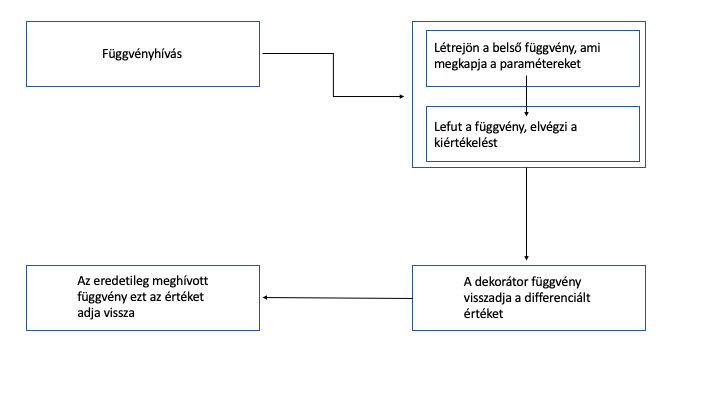
\includegraphics[width=\textwidth]{plots/numerical_derivation_decorator_explanation.png}
    \caption{Dekorátorok Pythonban (forrás: saját készítés)}
    \label{python_dekorator}
\end{figure}

Természetesen ha kidekoráltunk egy függvényt, akkor az már innentől kezdve végig a dekorált változatával fog működni. Tehát ha volt egy
\begin{equation*}
    f(x) \rightarrow 2x
\end{equation*}
függvény, amit dekoráltunk mondjuk a
\begin{equation*}
    g(x) \rightarrow x + 1
\end{equation*}
leképezéssel, akkor az új függvény neve f marad, de a funkcionalitása a következő lesz:
\begin{equation*}
    f' = g(f(x)) \rightarrow 2x + 1
\end{equation*}
Ennek majd egy nagyon praktikus példáját a Numba csomag használatakor látjuk, mert ott létrehozzuk az új, dekorált függvényt és azzal fogunk tovább dolgozni mindenféle egyéb probléma nélkül az elnevezéseket illetően.
\subsection{Python csomagok}
Mint minden nyelvben, itt is tudunk importálni már készen levő csomagokat, amelyek tartalmaznak a célnak megfelelő osztályokat, azon belül metódusokat. Ha nincs feltelepítve a csomag, akkor a \textbf{pip install csomag-neve} paranccsal tehetjük meg azt.
Amint ezt megtettük, az \textit{import csomag-neve as alias-csomag-neve} módon importálhatjuk a kódunkba. A könnyebb olvashatóság érdekében szokás \textit{alias}-t használni, de nem szükséges.

\lstinputlisting[language=Python]{python-bevezetohoz-scriptek/import_template.py}
Amennyiben a beépített pip csomagkezelőjét használjuk a Pythonnak, akkor érdemes megismerkedni a következő paranccsal:
\begin{lstlisting}[language=bash]
    pip list
\end{lstlisting}
Ezt használva ki tudjuk listázni, hogy milyen csomagokat telepítettünk fel és azok épp milyen verziószám alatt működnek. \newline
Ha esetleg törölni szeretnénk egy csomagot, akkor a
\begin{lstlisting}[language=bash]
    pip uninstall csomag
\end{lstlisting}paranccsal tehetjük meg. Persze az is előfordulhat, hogy valamilyen okból kifolyólag nem jó egy csomag verziója és nekünk specifikusan egy csomag egy adott verziójára van szükségünk, ezt a következő paranccsal tehetjük meg :

    \begin{lstlisting}[language=bash]
  pip install csomag == verzioszam
\end{lstlisting}
Ha pedig felvan sorolva egy .txt fájlban esetleg, hogy milyen csomag igénye van a környezetnek akkor elég a következő sor :
\begin{lstlisting}[language=bash]
pip install -r requirements.txt
\end{lstlisting}
, amennyiben a szöveg fájl neve reguirements.txt . \newline
Azonban van egy elterjedt és hasznos csomagkezelő, az Anaconda. Itt nagyon hasonló parancsokkal lehet csomagokat telepíteni, általában\cite{Anaconda} annyi a külöbség, hogy a pip szó helyett conda-t kell írni.
\begin{lstlisting}[language=bash]
conda install numpy
\end{lstlisting}
Az Anaconda főleg olyan emberek körében elterjedt, akik nem szeretnek a különböző csomagokkal foglalkozni, hanem azt szeretnék, hogy minden meglegyen egyben. Emiatt is népszerű az adattudósok körében az Anaconda. Ezen felül ha feltelepítjük az Anacondát, akkor lehetőségünk lesz használni a jupyter notebookot, illetve a JupyterLabot, amelyekben soronként lehet futtatni a Python szkripteket. Ez hatalmas nagy előny minden olyan ember számára, aki a Pythonnak olyan csomagjait szeretné használni, amelyekkel ábrákat készíthet (pl. matplotlib), statisztikai mutatókat számolhat vagy gépi tanulásos algoritmusokat szeretne futtatni.
\subsubsection{Numpy}
A NumPy a Python egy nagyon elterjedt és hasznos csomagja, ami nagy múltra tekint vissza. Amikor létrejött a Python, akkor  népszerűségre tett szert olyan emberek között, akik sok számításigényes kódot írtak (mert egyszerű volt - ahogy most is). 1995-ben megalkották a Numeric csomagot, aminek több beceneve is volt : Numerical, Numerical Python, NumPy. 2001-ben a különböző Numeric könyvtárakat egybedolgozták és létrejött a SciPy (Scientific Python), és nemsokra rá létrejött a "numarray" párhuzamosan. Mivel sokáig párhuzamosan fejlesztették a két könyvtárat sok, kompatibilitási probléma adódott, emiatt pedig 2005-ben ezt a kettő ágat összeforrasztották és ekkor jött létre a NumPy, már hivatalosan is NumPy néven. Azóta is ezen a néven fut. A NumPy használatában törekedni kell arra, hogy oszlopműveleteket használjunk, mert így tud "optimálisan" működni. Ez azt jelenti, hogy skalár és mátrix műveletekre nem lesz gyorsabb a futás várhatóan, de ha ezt oszlopműveletekben fogalmazzuk meg akkor gyorsabb lesz. Ennek az az oka, hogy amikor elküldjük a NumPy scriptet, akkor ezt "besorolja" a csomag és C/C++ kódot generál belőle olyan módon, hogy azokra már meglévő és optimális algoritmusokat fog használni (és ettől lesz gyorsabb). Miután legenerálta ezeket az alacsonyabb szintű kódokat, akkor azt már gyorsan le tudja fordítani gépi kódra a processzornak a compiler. Ehhez a "generáláshoz" önmagától is készít alacsonyabb szintű kódokat, azonban akárcsak a Matlab, az Octave vagy az R használja az ún. BLAS (Basic Linear Algebra Subprograms), LAPACK(Linear Algebra Package) specifikációkat, amelyekben leírtak és megalkottak optimális algoritmusokat a különböző algebrai műveletekre alacsony szintű nyelvekben, amelyek használata nagyban megkönnyíti a munkáját a különböző magasabb szintű nyelvek fejlesztőinek.
\begin{figure}[!h]
    \centering
    \includegraphics[width=\textwidth]{kepek/BLAS.jpg}
    \caption{NumPy működése, (forrás: saját készítés)}
    \label{Numpy működése}
\end{figure}

Ha esetleg nem oszlopműveletekre kihelyezett módon írjuk meg a szkriptünket, akkor nem a fent bemutatott gyorsabb módon megy végbe a futás, hanem a sima Python megoldásokat fogja használni, ami valószínűleg lassabban szolgáltat eredményt. Nem várható el, hogy magától felismerjen helyzeteket a nyelv ,és átírja a sorokat olyanra, amit hamarabb el tud végezni.\newline
Ilyen oszlopművelet lehet egy for ciklus például. Tegyük fel, hogy az a feladat, hogy egy számlista elemeit négyzetre kell emelni, majd kivonni belőle 1-et. Nézzünk meg erre egy NumPy mentes Python implementációt és egy NumPyos implementációt:
\pagebreak
\lstinputlisting[language=Python]{python-bevezetohoz-scriptek/numpy_examples.py}
Az első esetben eredeti python listát hoztunk létre a range() függvénnyel, majd egy ciklussal mentünk végig az elemeken és végeztük el a műveleteket. A második esetben pedig a range() függvény NumPyos változatát, az arange() függvényt használva hoztuk létre a listát, majd a power() függvénnyel emeltük négyzetre és abból vontunk ki 1-et belőle. Itt látszik véleményem szerint, hogy akkor tudunk valóban optimálisabb szkriptet írni, ha figyelünk arra, hogy törekedjünk az oszlopműveletekre, amikor Pythonban olyan üzleti igényt fejlesztünk, ami számításigényes.\newline
A 2 megoldást, mint látható is, ezerszer ismételtem meg és ezekből az eredményekből vontam átlagot.\newline


\begin{table}[H]
\caption{Vanilla Python és NumPy összehasonlítása (forrás: saját készítés)}
\centering
\begin{tabular}{|l|l|l|}
\hline
Python      & Numpy       & Arány    \\ \hline
2.62588e-04 & 3.38959e-06 & 77.46880 \\ \hline
\end{tabular}
\end{table}
Természetesen minden futáskor más lesz az eredmény, de többszöri ellenőrzés után az arány sosem ment 70 alá azon a számítógépen, amin ezeket a számításokat végeztem.

\subsubsection{Matplotlib}
A Matplotlib egy olyan Python csomag, ami leginkább kétdimenziós ábrák renderelésére hoztak létre. A megalkotója John Hunter Matlabban dolgozott már egy huzamosabb ideje és elkezdte érezni a szoftver limitációit. Ebből a felismerésből jött számára az ötlet, hogy egy olyan Python ojektumokkal kompatibilis csomagot hozzon létre, amivel kitudja váltani a fizetős Matlabot, ami akkoriban egyedülálló eszköz volt a 2D-s ábrák készítéséhez. Egy ábra úgy jön létre (renderelődik), hogy több rétegből tevődik össze, akárcsak amikor egy festő vagy grafikus létrehozza a munkáját. A művész is kigondolja, miről fog festeni, majd elkezdi felfesteni a különböző rétegeket a vászonra. Ez is hasonló módon történik meg a Matplotlib csomagban. Nagy vonalakban 3 réteg az, ami létrehozza az ábránkat. A legfelső réteg (Scripting) egy felhasználóbarát módon bekéri az adatokat a programozótól és ezt átalakítja a következő réteg számára. Gyakorlatilag ez a réteg jelenti magát a Matplotlib szkriptet, amit lefutattunk. Amikor ez megtörtént, eljutunk a középső (Artist) réteghez, ami a fentől kapott utasításokat átalakítja olyan formátumúvá, amelyet a kövekező (Backend) réteg már le fog tudni renderelni. Ez azt jelenti, hogy a festőecset a Backend réteg, mert itt kerül fel az ábra a vászonra. Az Artist réteg a festő keze, ami elviszi az ecsetet a vászonig és a Scripting réteg pedig a festő gondolata. Röviden itt is azt láthatjuk, mint pl. a NumPy esetén, hogy a Python szkript, amit megírunk több lépcsős folyamatban alakítódik át alacsonyabb szintű nyelvre.\newline
A szakdolgozatban a Scripting réteg a matplotlib.pyplot osztály, ez az amivel az ábrákat készítettem.
A következő ábrát például ezzel a kóddal generáltam le.
\begin{figure} [!h]
    \centering
    \includegraphics[width=\textwidth]{kepek/pyplot_example.png}
    \caption{Matplotlib példa (forrás: saját készítés)}
    \label{Matplotlib_pelda}
\end{figure}

Úgy működik a plot készítés, hogy a plt osztály különböző attribútumait feltöltjük a saját értékeinkkel, majd megjelenítük a plt.show() hívással. Ezeket pedig jól láthatjuk az alábbi kódban.

\lstinputlisting[language=Python]{python-bevezetohoz-scriptek/matplotlib_examples.py}
\section{Numerikus integrálás}
A numerikus integrálás nagyon fontos része a numerikus módszereknek. Egyrészről gyorsabban megkaphatjuk a határozott  integrál értékét, másrészről vannak olyan függvények, amelyeknek nem tudjuk kiszámolni papíron az integrál értéket, csak becsülni tudjuk alulról és/vagy felülről. A numerikus integrálás nagyban támaszkodik a kvadratúra képletekre.
\begin{definition}
Kvadratúra képletek általánosan

Az integrál értékét tudjuk közelíteni az ún. \textit{Kvadratúra képlettel}.\newline
\begin{equation*}
    \int_{a}^{b} f(x) dx \approx \sum_{k = 0}^{n} c_k f(x_k) = \sum_{k=0}^n \sigma_k \;\; , ahol\;\; x_i \in [a,b]
\end{equation*}

\end{definition}

Most nézzünk meg néhány kvadratúra képletet.
\subsection{Newton - Cotes formula}


Az integrálni való halmazt osszuk fel egyforma hosszúságúra, így vegyünk ekvidisztáns alappontokat.

\begin{equation*}
    x_k = a + hk \;\;, \;\;ahol \;\;k=0,1,...,n ,\;\; h = \frac{b-a}{n}
\end{equation*}
Írjuk fel a Lagrange - interpolációs kvadratúra képletet.
\newline
\begin{equation*}
    c_k = \int_a^{b} l_k(x) dx = h \int_0^{n} l_k (a+ht) dt = \frac{b-a}{n} \int_0 ^{n} \Pi_{j=0, j \neq k}^n \frac{t-j}{k-j} dt
\end{equation*}
Folytatva az egyenlőséget kapjuk, hogy
\begin{equation*}
   c_k =  \frac{b-a}{n} \frac{1}{k! (n-k)!} \int_0^n \Pi_{j=0}^{k-1} (t-j) \Pi_{j=k+1}^{n} (j-t) dt
\end{equation*}
\subsection{Összetett kvadratúra képlet}

\begin{equation*}
 \int_a^{b} f(x) dx = \sum_{j = 1} ^{m} \int_{a_{j-1}} ^{a_j} f(x) dx
\end{equation*}
 ahol $a_0 = a, a_m =b $

A baloldali részintegrált írjuk fel az interpolációs kvadratúra képlettel:
\begin{equation*}
\int_{a_{j-1}}^{a_j} f(x) dx \approx \sum_{k=0}^{r} c_{k,j}f(x_{k,j})
\end{equation*}

Innen helyettesítsünk vissza az eredeti képletbe
\begin{equation*}
\int_a^b f(x) dx \approx \sum_{j=1}^{m} \sum_{k=0}^{r} c_{k,j} f(x_{k,j})
\end{equation*}


\subsection{Érintő formula}

Az érintő formulához fel tudjuk használni a függvények lineáris Taylor közelítését. Ezen felül vegyük az intervallum ekvidisztáns felosztását.
\begin{equation*}
   x_k = a + (k - \frac{1}{2})h ,\;\; ahol\;\; h = \frac{b-a}{n},\;\; k =1,...,n.
\end{equation*}



A Taylor közelítése a függvénynek a $[x_k-\frac{h}{2},x_k+\frac{h}{2}]$ intervallumon
\begin{equation*}
    f(x) \approx f(x_k)+f'(x_k)(x-x_k).
\end{equation*}

\begin{equation*}
\int_{x_k-\frac{h}{2}}^{x_k + \frac{h}{2}} \approx \int_{x_k - \frac{h}{2}}^{x_k + \frac{h}{2}} [f(x_k) + f'(x_k)(x-x_k)] dx = hf(x_k)
\end{equation*}
\newline
Innen pedig kapjuk, hogy
\begin{equation*}
\int_a^b = f(x) dx = \sum_{k=1}^n \int_{x_k - \frac{h}{2}}^{x_k + \frac{h}{2}} f(x)dx \approx h \sum_{k=1}^n f(x_k)
\end{equation*}



\subsection{A trapéz módszer és a Newton - Cotes módszer}
Írjuk fel a Newton - Cortes formulát n = 1 és k = 0 melett:
\begin{equation*}
c_0 = \frac{b-a}{1} \frac{1}{0!(1-0)!} \int_0^{1} \Pi_{j=0}^{0-j} \Pi_{j=0+1}^{1} (j-t) dt = (b-a) \int_0^1 (1-t) dt = \frac{b-a}{2}
\end{equation*}

\begin{equation*}
c_1 = \frac{b-a}{2}
\end{equation*}
Ekkor

\begin{equation*}
    \int_a^b f(x) dx \approx \frac{b-a}{2}[f(a) + f(b)] = \sum_{k=0}^{1} \frac{b-a}{2} f(x_k),\\
    \;\;ahol \;\;x_0 = a,\;\;x_1=b
    \;\;
\end{equation*}

Ez pedig pont a trapéz területe! Nézzünk erre egy példát :
\newline
\begin{figure}[!h]
    \centering
    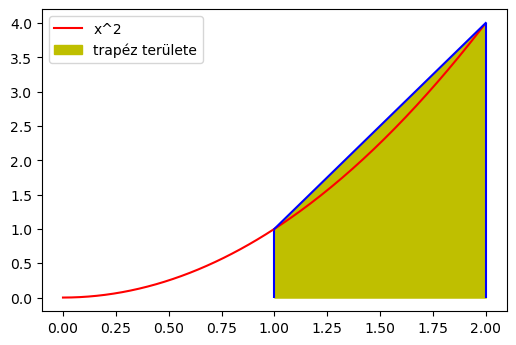
\includegraphics{plots/trapez_with_area.png}
    \caption{Trapéz módszer, (forrás: saját készítés)}
    \label{trapez_pelda}
\end{figure}


Az integrál értéke ezen az intervallum 7/3.
\begin{center}
$\int_{1}^{2} x ^2 dx = \frac{7}{3}$
\end{center}
Azonban, ha ezen paraméterek között végezzük el a trapéz - területszámítást akkor 2.5 - t kapunk eredményként. Ezt onnan is láthatjuk, hogy a fenti ábrán a kék és piros vonal között még akad zöld terület. Azonban most számoljuk ki ezzel a módszerrel az integrál értékét az [1,1.5] és [1.5,2] intervallumokon. Ekkor eredményül 0.8125 és 1.5625, összesen 2.375 értéket kapunk, ami közelebb van a 7/3-hoz

\begin{figure}[h]
    \centering
    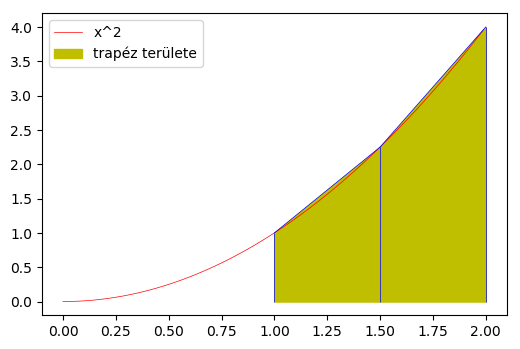
\includegraphics{plots/trapez_n=2.png}
    \caption{Finomított trapéz beállítás (forrás: saját készítés)}
    \label{n=2_trapez_pelda}
\end{figure}
\pagebreak

\subsection{Python kódok a fejezethez}
A trapéz függvényben használjuk a globals() metódust. Ez a metódus visszaadja az összes olyan objektumot, amely az adott programunk futásakor belekerült a compilerbe(fordítoprogram). Ezek között lesznek azok a függvények, amiket megírtunk. A globals() egy dictionaryt ad vissza, amiben mi a függvény nevét fogjuk használni, mint kulcs. Ez azért hasznos számunka, mert minden függvényt megtudunk hívni a nevével, mint paraméter. Eszerint tudunk olyan függvényt írni, aminek egy paramétere egy másik függvény. A limitációi ennek a módszernek többek között az, hogy csak fájlon belül fog működni. Ha a külső függvény nem egy modulban szerepel azzal a függvénnyel, amiben pont a kalkulációt írtuk meg, akkor a külső függvény a globals() metódusból egy olyan listát fog megkapni, ami a vele egy helyen szereplő függvények nevei. Itt pedig könnyen 'KeyError'-t kaphatunk.
\pagebreak
\lstinputlisting[language=Python]{functions.py}
\pagebreak
\section{Szukcesszív approximációs módszer}

\begin{definition}{ODE}\\
Közönséges differenciálegyenletnek(Ordinary Differential Equation) nevezzük azokat az egyenleteket, amelyekben szerepel egy x függvény egy változója szerinti deriváltja és célunk meghatározni az x függvényt.\\
Például
\begin{equation*}
    \frac{dx}{dt} (t) = cos(t)
\end{equation*}
\end{definition}

\begin{definition}Autonóm differenciálegyenlet\\
Írjuk fel a következő ODE-t:
\begin{equation*}
    f(x,y) = \frac{dx}{dt} = x'
\end{equation*}
Azokat a differenciálegyenleteket nevezzük autonómnak, amelyek nem függnek az x változótol a fent leírt egyenletben.Általánosan így néz ki egy autonóm egyenlet.
\begin{equation*}
    \frac{dx}{dt} = f(x)
\end{equation*}
Ha t paramétert az időnek vesszük, akkor ebben az egyenletben azt láthatjuk, hogy nem függ az időtől az y megváltozása, mindig állandó a deriváltja, f(y) a változás időtől függetlenül.
\end{definition}

\begin{definition}Lineáris differenciálegyenlet\\
Lineáris differenciálegyenletnek nevezzük azokat a differenciálegyenleteket, ahol a jobb oldali f függvényt feltudjuk írni x deriváltjainak lineáris kombinációjaként.
Példa erre a következő:
\begin{equation*}
    a_1 x'(t) + a_2 x''(t) = f(t)
\end{equation*}
\end{definition}

\begin{definition}Homogén lineáris differenciálegyenlet\\
Ha a fenti lineáris differenciálegyenlet jobboldala azonosan nulla, homogén lineáris differenciálegyenletnek nevezzük.Ha a jobboldal nem azonosan nulla, akkor az egyenletet inhomogén lineáris differenciálegyenletnek nevezzük.
\end{definition}
\begin{definition}{Kezdetiérték-feladat}\\
Vegyünk egy ODE problémát és adjunk meg hozzá egy (kezdeti) pont-függvény párost. Az ODE-t ezzel a tulajdonsággal ellátva kezdetiérték problémának  nevezzük
\begin{equation*}
    \begin{cases}
       x'(t) = f(t,x(t))\\
       x(t_0) = x_0 \\
    \end{cases}
\end{equation*}
\end{definition}
\begin{definition}{Lipschitz folytonosság}

\begin{equation*}
Legyen \;\;    f : \mathbb{R} \rightarrow \mathbb{R}, \; és \;\; L\; \;\in \mathbb{R}^+
\end{equation*}

Ha f minden x és y pontjára fennáll a következő
\begin{equation*}
    |f(x) - f(y)| \leq L |x-y|
\end{equation*}
egyenlőtlenség, akkor \textit{Lipschitz folytonosnak} nevezzük az f függvényt
\end{definition}
\begin{definition}{Kontrakció}\\
Legyen (X,$\textit{d}$) egy teljes metrikus tér. T leképezést $\textit{kontrakciónak}$ nevezzük X alaphalmazon, ha $\exists$ $q \in [0,1)$, hogy
\begin{equation*}
    d(T(x),T(y)) \leq q \textit{d}(x,y) \;\;,\forall x,y \in X
\end{equation*}
Pongyolán fogalmazva ezt jelenti, hogy azok a  Lipschitz folytonos függvények a kontrakciók, amelyekben az L Lipschitz konstans kisebb 1-nél.
\end{definition}
\begin{theorem}[Banach-féle fixponttétel]
Legyen (X,$\textit{d}$) egy nemüres, teljes metrikus tér ellátva egy T kontrakcióval. Ekkor
\begin{equation*}
    \exists!\;\; x^* \in X : T(x^*) = x^*
\end{equation*}
\end{theorem}
\begin{proof}
Részletesen nem tisztázzuk a tétel bizonyítását, csak megemlítjük a főbb lépéseket.

\begin{equation*}
Legyen\;\;(X_n)_{n \in \mathbb{N}},\;\; x_n = T(x_{n-1}), \;\;x_0 \in X \;\;egy \;\; sorozat
\end{equation*}
Mivel T kontrakció, így igaz a következő egyenlőtlenség
\begin{equation*}
    d(x_{n+1},x_n) \leq q^n d(x_1,x_0)
\end{equation*}
Ha ezeket felhasználva elkezdünk \textit{n}-ben iterálni, könnyű belátni, hogy
\begin{equation*}
    \forall \;\; \epsilon >0 \;\; számhoz \;\; van \;\; olyan \;\; k_0 \;\;küszöbindex,\;\;hogy\;\; \forall j,k \geq k_0 \;\;esetén \;\;;d(x_j,x_k) j < \epsilon, \;\;j\neq k  \;\;
\end{equation*}
azaz  $(x_n)$ Cauchy  sorozat.
Mivel az (X,d) metrikus tér teljes, ezért a sorozatunknak létezik határértéke, sőt ez a határéték pont T leképezés fix pontja lesz. A fix pont egyértelműségét igazolhatjuk, ha indirekt feltesszük, hogy van másik fix pont.
\end{proof}
%https://en.wikibooks.org/wiki/Ordinary_Differential_Equations/The_Picard–Lindelöf_theorem
\begin{theorem} [Picard - Lindelöf] \\
Legyen I =[a,b] egy intervallum , és egy f függvény,

\begin{equation*}
f :  I \times \mathbb{R}^n \rightarrow \mathbb{R}^n
\end{equation*}
Legyen x' pedig egy ODE
\[
x'(t) = f(t,x(t))
\]
Ha f Lipschitz folytonos x(t)-ben, akkor az ODE-nek létezik egyértelmű megoldása [a,a + $\epsilon$]
intervallumon minden
\[
x(0) = x_0 \in \mathbb{R}^n, \epsilon < \frac{1}{L}
\] halmazra és L pedig x(t) Lipschitz konstansa
\end{theorem}
\begin{proof}
Írjuk fel ezt egy kezdeti-érték feladatra
\begin{equation*}
    \begin{cases}
       f :  I \times \mathbb{R}^n \rightarrow \mathbb{R}^n , t \in [a,a + \epsilon]\\
       x'(t) = f(t,x(t))\\
    \end{cases}
\end{equation*}

Ez a Newton - Leibniz tétel miatt pedig erre az alakra hozható:
\begin{equation*}
    \forall t \in [a, a +\epsilon] : x(t) = x_0 + \int_{a}^{t} f(s,x(s)) ds
\end{equation*}
 ahol pedig $\epsilon < \frac{1}{L}$. Eszerint x(t) fixpontja a következő függvénynek :

 \begin{equation*}
     T : \mathcal{C}([a, a +\epsilon]) \rightarrow \mathcal{C}([a, a +\epsilon]), T(x,t) := x_0 + \int_a^t f(s,x(s)) ds
 \end{equation*}
 T kielégíti a Lipschitz folytonosságot, mivel
 \begin{equation*}
    \begin{split}
     \lVert T(x,t) - T(y,t) \rVert =\lVert \int_a^t f(s,x(s)) ds - \int_a^t f(s,x(s)) ds \rVert &
     \leq \int_a^t \lVert f(s,x(s)) - f(s,y(s)) \rVert ds \leq \int_a^t L \lVert x(s) - y(s) \rVert &
     \leq (t-a) L \lVert x-y\rVert_{\infty} \leq \epsilon L \lVert x - y \rVert_{\infty}
     \end{split}
 \end{equation*}

 Mivel T pedig kontrakció, így a Banach-féle fixpont tétel alkalmazható,amivel igazoltuk a létezését a megoldásnak. Továbbá felhasználva a Peano-egyenlőtlenséget megkapjuk az egyértelműséget is.
\end{proof}
\begin{definition}[Szukcesszív approximációs módszer]
Vegyük a következő kezdetiérték problémát
\begin{equation*}
    \begin{cases}
       x'(t) = f(t,x(t))\\
       x(a) = b
    \end{cases}
\end{equation*}
Fentebb tárgyaltuk a Picard-Lindelöf tételnél, hogy a Newton - Leibniz tétel miatt fennáll a következő
egyenlőség: \newline
\begin{equation*}
    x(t) = x(0) + \int_a^t f(s,x(s)) ds
\end{equation*}
Ekkor vegyük az \[x_0(t) = b\] állandót, majd kezdjünk el előre iterálni a következő képlet alapján:
\begin{equation*}
    x_{n + 1}(t) = b + \int_a^t f(s,x_n(s)) ds
\end{equation*}
\end{definition}

\begin{example}[Exponenciális függvény]
\begin{equation*}
    \begin{cases}
       y'(t) = y\\
       y(0) = 1
    \end{cases}
\end{equation*}
Kezdjünk el lépkedni.
\begin{equation*}
    y_1(t) = 1 + \int_0^x 1 dt = 1 + x
\end{equation*}
\begin{equation*}
    y_2(t) = 1 + \int_0^x 1+t dt = 1 + x + \frac{x^2}{2}
\end{equation*}
\begin{equation*}
    y_3(t) =  1 + x + \frac{x^2}{2} + \frac{x^3}{6}
\end{equation*}
\begin{equation*}
    y_4(t) = 1 + x + \frac{x^2}{2} + \frac{x^3}{6} + \frac{x^4}{24}
\end{equation*}
\begin{equation*}
    y_{\infty}(t) = exp(x)
\end{equation*}
\end{example}
\subsection{Python kódok a fejezethez}
\lstinputlisting[language=Python]{fokozatos_kozelitesek/successive.py}
\section{Runge-Kutta módszer}
A Runge-Kutta algoritmusok az egyik legelterjedtebb megoldó módszerek a numerikus analízis eszköztárában, mivel 'olcsó' a használatuk, nem igényelik a függvények deriváltjainak az ismeretét és mégis elfogadható pontossággal műküdnek (ez például nem mondható el feltétlen az Euler módszerről). A módszer a nevét két német matematikusról kapta, névszerint Carl Runge és Wilhelm Kuttáról.

\subsection{Euler módszer}
Az Euler módszer az alapja a numerikus differenciálegyenlet megoldó módszereknek, azonban nem hatékony a használata, mert lassabban konvergál a megoldáshoz, mint például a Runge-Kutta módszer. Ettől függetlenül érdemes megvizsgálni a módszert, mert szemléletes és korlátozottan, de működőképes.

Vegyünk egy kezdetiérték problémát és hozzá egy lépésközt.
\begin{equation*}
    \begin{cases}
       x'(t) = f(t,x(t))\\
       x(a) = b \\
       t_i = a + ih , i \in \{0,1,...,N\}
    \end{cases}
\end{equation*}

Itt pedig a lépésköz pedig legyen \[h = \frac{b-a}{N} = t_i - t_{i-1} \] .

Használjuk fel a Taylor sorbafejtést másodrendben x-re.
\begin{equation*}
    x(t_{i+1}) = x(t_i) + h x'(t_i) + \frac{h^2}{2} x''(\xi_i) \;\;,\;ahol \;\;\xi _i \in (t_i, t_{i+1})
\end{equation*}

Ezek alapján pedig láthatjuk, hogy az algoritmust a következőképpen írhatjuk fel:
\begin{equation*}
    \begin{cases}
        x_0 = \alpha \\
        x_{i+1} = x_i + h f(t_i,x_i) \;\;\forall i \in{0,1,...,N-1}
    \end{cases}
\end{equation*}
\subsection{RK4}
Runge - Kutta módszerekből sokat alkottak az utóbbi időkben. Ha egyszerűen próbáljuk meg megközelíteni ezeknek a megoldó algoritmusoknak a felépítését, akkor észrevehetjük, hogy ahányad rendű Runge - Kutta módszert használunk, annyiad rendű Taylor sor közelítést használunk.Mi most a Runge-Kutta negyedfokó közelítését használjuk, amire a szakirodalomban sokszor csak 'RK4' módon hivatkoznak. A 4-ed rendű közelítés a következő formulából vezethető le:
\begin{equation*}
\begin{split}
      y_{t+h} = y_t + h \sum_{i=1}^{s} a_i k_i + \mathcal{O}(h^{s+1}),\\
      ahol\;\;k_i = y_t + h \sum_{j=1}^{s} \beta_{i,j} f(k_j,t_n + \alpha_ih)
\end{split}
\end{equation*}

A képlete pedig s=4 mellett:
\begin{equation*}
\begin{cases}
        x_0 = \alpha \\
        k_1 = h f(t_i,w_i) \\
        k_2 = h f(t_i + \frac{h}{2}, w_i + \frac{1}{2} k_1) \\
        k_3 = h f(t_{i + 1} + \frac{h}{2}, w_i + \frac{1}{2} k_2) \\
        k_4 = h f(t_{i + 1}, w_i + k_3)\\
        w_{i+1} = w_i + \frac{1}{6}(k_1 + 2k_2 + 2k_3 + k_4)\\
        t_{i+1} = \alpha + ih
\end{cases}
\end{equation*}
Ezt pedig már tudjuk iterálni i-ben egy rögzített h mellett. Ennek a közelítésnek előnye, hogy a hibahatára már elfogadható és nem igényel annyira sok számítást, mint egy magasabb rendű közelítés.
\subsection{Példa feladatok}
\begin{example} [Konstans együtthatós lineáris ODE]
Legyen \\
\begin{center}
   \begin{cases}
    x' = 5x - 3 \\
    x(0) = 1
   \end{cases}
\end{center}
Ennek a kezdetiérték feladatnak az analitikus megoldása a következő:
\begin{equation*}
\begin{split}
        \frac{dx}{dt} &= 5x - 3 \\
        \frac{1}{5x-3} dx &= 1\; dt \\
        \int \frac{1}{5x-3} dx &= \int 1\; dt \\
        \frac{1}{5} ln|5x-3| &=t + C \\
        5x -3 &=e^{5(t + C)} \\
        x &= \frac{e^{5(t+C)} + 3}{5}
\end{split}
\end{equation*}
Mivel x(0) = 1, így
\begin{equation*}
    x(0) = \frac{e^{0+C} + 3}{5} = \frac{e^{5C}+3}{5} = 1
\end{equation*}
\begin{equation*}
    e^{5C} + 3 = 5
\end{equation*}
\begin{equation*}
    5C = ln2
\end{equation*}
\begin{equation*}
    C = \frac{ln2}{5}
\end{equation*}
Tehát a keresett függvény :
\begin{equation*}
    x(t) = \frac{e^{5(t + \frac{ln2}{5})} + 3}{5}
\end{equation*}
Nézzük meg mennyit ad a függvény a t=1 pontban:
\begin{equation*}
    x(1) = \frac{e^{5(1 + \frac{ln2}{5})} + 3}{5} \approx 59.9653
\end{equation*}
A függvényünk h = 0.1-es lépésköz mellett 59.8632 -es értéket adott. Ha h = 0.01, akkor sok tizedesjegyig megegyezik az eredmény. Azonban nem feltétlen szabad a megoldó algoritmusban h - t igazán kicsinek venni, mert könnyen a visszajára fordulhat. (Ez például függ attól, hogy hány bites a processzor. Nagyon nagy irodalma van az optimális értékek beállítására, azonban most ez a szakdolgozat ezzel nem foglalkozik).
\end{example}

\begin{example}[Folytonos kamatozás]
Tegyük fel, hogy elhelyezünk egy bankban konstans kamatláb mellett egy betétet folytonos kamatozás mellett. Tudjuk, hogy a folytonos kamatozás képlete
\begin{equation*}
    e^{rt},\;\; ahol \; r\; a\; kamatláb \;és\;t\; az \;idő.
\end{equation*}
Ezt kifejezhetjük egy kezdetiérték probléma alakban is a következő módon : \\
\begin{center}
  \begin{cases}
        x' = rx \\
        x(0) = 1
  \end{cases}
\end{center}
Ennek a megoldása pedig pont visszaadja a fentebb írt képletet: \\
\begin{equation*}
    \frac{dx}{dt} = r x
\end{equation*}
\begin{equation*}
    \frac{1}{x} dx = r dt
\end{equation*}
\begin{equation*}
    \int \frac{1}{x} dx = \int r dt
\end{equation*}
\begin{equation*}
    ln|x| = rt + c
\end{equation*}
\begin{equation*}
    x = e^{rt + c}
\end{equation*}
Mivel a kezdeti feltétel x(0) = 1, így c = 0 és visszakapjuk az eredeti képletet\\

Nézzük meg mennyi lehet x(1) értéke, úgy hogy r = 0.1 a kamatláb. A képlet szerint tudjuk, hogy
\begin{equation*}
    e^0.1 = x(1) = 1.105170918...
\end{equation*}
Ha ezt az értéket beheleyttesítjük a numerikus RK4-es függvényünkbe, akkor az x(1) = 1.1051709180665144 eredményt kapjuk 0.1-es lépésköz mellett. Ennél példánál a negyedrendű Runge-Kutta módszer elég pontos eredményt adott
\end{example}


\begin{example}[Másik példa]\\
Legyen \\
\begin{center}
   \begin{cases}
    x' = \frac{x^3}{3} \\
    x(0) = 3
   \end{cases}
\end{center}
egy kezdeti érték feladat. Ennek a megoldása pedig
\begin{equation*}
    x(t) = \frac{3}{\sqrt{1-6t}}
\end{equation*}

Az analitikus eredmény t = 0.1 pontban :
\begin{equation*}
    x(0.1) \approx 4.7434
\end{equation*}
A Runge-Kutta módszer eredménye úgyszintén 4.7434.
\end{example}

\begin{example} [Egy nehezebb elsőrendű feladat]
Nézzük a következő feladatot: \\
\begin{center}
    \begin{cases}
     x' = \frac{1}{x(9 + 4 t^2)} \\
     x(0) = 1
    \end{cases}
\end{center}
Ennek a feladatnak az analitikus megoldása :
\begin{equation*}
    x(t) = \sqrt{\frac{1}{3} arctg(\frac{2t}{3}) + 1}
\end{equation*}
\begin{equation*}
   x(0) = \sqrt{\frac{1}{3} arctg(\frac{0}{3}) + 1} = 1
\end{equation*}
A numerikus eredmény pedig: 1.0110.
Ez az első feladat, ahol jelentős az eltérés, nevesen kb. 0.01
\end{example}
A Runge-Kutta és minden egyéb numerikus módszer tehát nem alkalmas a függvény formájának analitikus módon történő képlettel való meghatározására, hanem egy közelítést ad arra, hogy mi lehet a keresett függvény \textbf{értéke az adott pontban.}
\subsection{Eredmények összevetése}
A Runge Kutta módszer kevesebb lépésből mindig pontosabb eredményt adott, ez is egy oka , amiért ez terjedt el inkább az oktatásban. Azonban most az egyszerűség kedvéért az Euler módszer eredményeit úgy közlöm ebben a táblázatban, hogy nem ugyanakkora energiabefektetéssel készültek, mint az RK4-es párjai. Ez a gyakorlatban azt jelenti, hogy minden esetben addig emelgettem az iterációs számokat, ameddig be nem állt az adott értékre, amitől már számottevően nem tért el a továbbiakban. Ezek után a legjobb Euler módszer eredményeket tettem bele a táblázatba, míg az RK4-es eredmények konzistensen nem változtak felépítésüket tekintve, nem nyúltam bele sehogy sem a megoldó algoritmus paramétereibe.
\begin{table}[H]
\caption{Numerikus algoritmusok performacia vizsgálata (forrás: saját készítés)}
\begin{tabular}{|l|l|l|l|}
\hline
                           & Analitikus megoldás & Runge Kutta & Euler módszer \\ \hline
Konstans együtthatós példa & 59.9653             & 59.9652     & 59.2302       \\ \hline
Kamatláb példa             & 1.1051              & 1.1051      & 1.1051        \\ \hline
Harmadfokú példa           & 4.7434              & 4.7434      & 4.7409        \\ \hline
Bonyolultabb példa          & 1.0000              & 1.0110      & 1.0936        \\ \hline
\end{tabular}
\end{table}
Látni az eredményeken, hogy az RK4 jobb eredményekre vezetett az Euler módszernél. A következő néhány képen pedig bemutatjuk a két módszer pontosságát. Az első képen a konstans együtthatós példa szerepel 100-as és 200-as lépésszámok mellett. Látni, hogy az RK4 kevesebb lépésből közelebb került a megoldáshoz.
\begin{figure}[!h]
    \centering
    \includegraphics[width=\textwidth, height=290pt]{RK4/plotok/konstans_rk4=100_euler=200.png}
    \caption{Runge-Kutta és Euler módszer különböző lépésszám mellett (forrás: saját készítés)}
    \label{Rk4_euler_1}
\end{figure}

A második képen pedig látni, hogy ugyanakkora lépésszám mellett ebben az esetben pedig pontosabb eredményt adott az RK4.
\begin{figure}[h]
    \centering
    \includegraphics[width=\textwidth]{RK4/plotok/konstans_mindketto_200.png}
    \caption{RK4 - Euler azonos lépésszám mellett (forrás: saját készítés)}
    \label{rk4_euler_pelda2}
\end{figure}


Természetesen úgy teljes, ha megmutatjuk, hogy más esetekben ezektől függetlenül nehéz leolvasni az ábráról, hogy van eltérés az eredmények között. Ilyen volt az a példa, ahol a kamatláb esetet vizsgáltuk. Itt a piros vonalat meg kellett vastagítani, mert végig fej fej mellett haladt a két vonal.\newline
\begin{figure}[H]
    \centering
    \includegraphics[width=\textwidth, height=290pt]{RK4/plotok/kamatlab_step=100.png}
    \caption{Kamatláb modell azonos lépésszám mellett (forrás: saját készítés)}
    \label{kamatlab_pelda}
\end{figure}

\pagebreak

\subsection{Magasabb rendű egyenletek megoldása}
A Runge Kutta módszerek alkalmazhatóak magasabb rendű differenciálegyenletek megoldására is. Alapvetően nagyon hasonlít az elsőrendű megoldó képlethez. Amikor analitikusan szeretnénk megoldani egy magasabb rendű egyenletet, akkor általában úgy szoktuk azt megtenni, hogy bevezetünk új változókat az egyes deriváltakra és ezt folytatva redukáljuk a problémát egy olyan feladatra, aminek már ismerjük a megoldási lehetőségét, lehetőségeit. Ha le tudtuk redukálni a problémát elsőrendű alfeladatokra, akkor azok össze lesznek kapcsolódva a bizonyos változókban és erre tudjuk alkalmazni például a Runge Kutta módszert (nem feltétlenül csak a negyed rendű közelítést).\newline
Nézzük meg példának egy (általánosan felírt) másodrendű differenciálegyenlet megoldását az RK4 módszerrel.
\begin{center}
    \begin{cases}
    x'' = f(t,x,x') \\
    x(t_0) = x_0 \\
    x'(t_0) = z_0
   \end{cases}
\end{center}
Vezessük be a következő változókat:
\begin{equation*}
    z = x'
\end{equation*}
\begin{equation*}
    z' = x'' = f(t,x,x') = f(t,x,z)
\end{equation*}

\begin{center}
    \begin{equation*}
        x = &
        \begin{bmatrix}
            x_n \\
            z_n
        \end{bmatrix}
    \end{equation*}
\end{center}
\begin{center}
    \begin{equation*}
        K_i = &
        \begin{bmatrix}
            K_i \\
            L_i
        \end{bmatrix}
    \end{equation*}
\end{center}
\begin{equation*}
    K_1 = h Z_n , \;\;L_1 = h f(t_n, x_n, Z_n)
\end{equation*}

\begin{equation*}
    K_2 = h (Z_n + \frac{L_{1}}{2}) , \;\;L_2 = h f(t_n + \frac{h}{2}, x_n+ \frac{K_{1}}{2}, Z_n + \frac{L_{1}}{2})
\end{equation*}

\begin{equation*}
    K_3 = h (Z_n + \frac{L_{2}}{2}) , \;\;L_3 = h f(t_n + \frac{h}{2}, x_n+ \frac{K_{2}}{2}, Z_n + \frac{L_{2}}{2})
\end{equation*}

\begin{equation*}
    K_4 = h (Z_n + L_{1}) , \;\;L_4 = h f(t_n + h, x_n+ K_{3}, Z_n + L_{1})
\end{equation*}

Ezután pedig a kettő megoldandó egyenletet az előbbiekhez  hasonlóan elkezdjük iterálni a következő képletek alapján:

\begin{equation*}
    x_{n+1} = x_n + \frac{1}{6}(K_1 + 2K_2 + 2K_3 + K_4)
\end{equation*}

\begin{equation*}
    Z_{n+1} = Z_n + \frac{1}{6}(K_1 + 2K_2 + 2K_3 + K_4)
\end{equation*}
\subsection{Python kódok a fejezethez}

Ebben az alfejezetben találjuk a Runge Kutta numerikus módszer implementációját elsőre, majd a második szkriptben a példa függvényeket és a megoldó függvény használatára példákat. Nézzük is meg elsőre magát a megoldó függvényt. Miután felsoroljuk a bemeneti változókat a dokumentációban eltudjuk olvasni, hogy mi mit is jelent. Meghatározódik n változóban a lépésszám, majd a globals() segítségével elkezdjük kiszámolni az adott konstansokat a különböző iterációs lépésekben és ezeken keresztül haladunk a numerikus megoldás felé.
\pagebreak
\lstinputlisting[language=Python]{RK4/rk4.py}

\lstinputlisting[language=Python]{RK4/rk4_examples.py}
\pagebreak
Itt pedig az Euler módszer általam megírt változatát találhatjuk.
\lstinputlisting[language=Python]{RK4/euler_method_template.py}
\section{Stabilitáselméleti kitekintés}
A stabilitáselmélet számottevő részét képezi a differenciálegyenletek témakörének. Ebben a dolgozatban szeretnénk egy kicsi betekintést nyerni ebbe a világba. Első körben tisztázzunk néhány definíciót.
\subsection{Alapfogalmak}
A fejezetben végig vegyük adottnak a
\begin{equation*}
    x' = f(t,x)
\end{equation*}
differenciálegyenlet, ahol
\begin{equation*}
    f: I \times \Omega \rightarrow \mathbb{R}^n \\
\end{equation*}
\begin{equation*}
    (t,x) \rightarrow f(x)
\end{equation*}
\begin{equation*}
    I=(t,\infty)
\end{equation*}
\begin{equation*}
    0 \in I
\end{equation*}
\begin{definition}[Egyensúlyi pont]
Egy f(a) = 0 tulajdonságú pontot a differenciálegyenlet egyensúlyi pontjának nevezzük.
\end{definition}
\begin{definition}[Stabilitás]
Legyen $x_0 \in \Omega$ egyensúlyi helye az egyenletünknek. Ekkor azt mondjuk, hogy $x_0$ egyensúlyi pont stabil, ha $\forall \epsilon > 0 $ számhoz létezik olyan $\delta > 0$ szám, hogy a kiinduló egyenlet minden $|x(0) - x_0| \leq \delta$ tulajdonságú megoldására minden $t \in \mathcal{D}_x \cup  [0, + \infty)$ esetén  $|x(t) - x_0| \leq \epsilon$
\end{definition}

\begin{definition}[Instabilitás]
Az instabil, ami nem stabil.
\end{definition}

\begin{definition}[Vonzás (attraktivitás)]
Az x' = f(t,x) x=0 megoldását vonzónak nevezzük, ha létezik
$\delta_0 > 0$ szám, hogy a kiinduló egyenlet bármely,  a nemnegatív félegyenes egészén értelmezett, $|x(0) - x_0| \leq \delta_0$ tulajdonságú megoldására fennáll a következő
\begin{equation*}
    \lim_{t \rightarrow + \infty} x(t) = x_0
\end{equation*}
határérték.
\end{definition}
\begin{definition}[Asztimptotikus stabilitás]
A kiinduló egyenlet megoldását aszimptotikusan stabilnak nevezzük, ha egyszerre stabil és vonzó
\end{definition}

\subsection{Lineáris algebrai kitekintő}
Amikor egy rendszer stabilitását vizsgáljuk, akkor nagyban kell támaszkodnunk a különböző lineáris algebrai ismereteinkre. Ezért a következőkben kimondunk néhány tételt és definíciót, amelyek segítenek megérteni a különböző tételeket, amelyek a stabilitásvizsgálathoz kapcsolódnak. Érdemes megemlíteni, hogy már fentebb beszéltünk a vektorműveletek hatékonyságáról, ami nagyban támaszkodik a lineáris algebra eszköztárára. Természetesen ezeknél a számításoknál is a NumPy csomag osztályaira hagyatkozunk, nevesen a linalg modulra.

\subsubsection{Mátrix az exponenciális függvényben}
Az egydimenziós exponenciális függvény és a mátrixokra kiterjesztett változata képletben nem mutat eltérést, sőt a különböző konvergencia megállapítások is hasonlítanak egymásra. Az alábbo fogalmak tisztázása szükséges a fejezet megértéséhez.
\begin{definition}[Mátrixokra kiterjesztett exponenciális függvény]
Legyen X egy négyzetes mátrix. Ekkor a következő módon értelmezzük a mátrix kitevőt az exponenciális függvényben.
\begin{equation*}
    exp(X) := \sum_{k=0}^{\infty} \frac{X^k}{k!}
\end{equation*}
\end{definition}
\begin{theorem}
A mátrixokra kiterjesztett exponenciáliss függvény tartja a következő tulajdonságokat:
        \begin{equation*}
            e^{A+B} = e^A  e^B
        \end{equation*}
        amennyiben AB = BA.
        \begin{equation*}
            e^{-A} e^{A} = I
        \end{equation*}
        Ahol I az egységmátrix.
        \begin{equation*}
            \frac{d}{dt} e^{tA} = A e^{tA}
        \end{equation*}
\end{theorem}
\subsubsection{Sajátértékek és sajátvektorok}
\begin{definition}[Sajátérték]
Legyen A egy lineáris operátor (mátrix). Vegyünk emellé egy nemnulla vektort. Ekkor a $ \lambda \in \mathbb{C}$ az A mátrix sajátértéke, ha kielégíti a következő egyenletet
\begin{equation*}
    Ax = \lambda x
\end{equation*}
Szokás átrendezni ezt az egyenletet és a következő formában megadni:

\begin{equation*}
    (A-\lambda I)x= \textbf{0},
\end{equation*}
ahol I természetesen az egységoperátor (mátrix)
\end{definition}
A lambda skalárt a komplex számok felett definiáltuk, hogy ne sértsük meg az általánosságot, de ez működik a valós számtest felett is (ami a komplex számtest részhalmaza).
\begin{definition}[Sajátvektor]
Legyen A egy lineáris operátor, jelesül egy mátrix .Az A mátrix minden olyan nem zérus \mathbb{x} vektorát sajátvektorának nevezzük, amelyre fennáll a következő egyenlőség
\begin{equation*}
    Ax = \lambda x
\end{equation*}
\end{definition}
A sajátvektor skalárszorosa is sajátvektor marad ugyanazzal a sajátértékkel.

Tehát a sajátérték és a sajátvektor fogalmak nagyon szoros kapcsolatban állnak egymással.

\subsubsection{Sajátértékek meghatározása}
Amikor meg kell határoznunk egy mátrix sajátértékeit, akkor azt alapvetően többféle képpen tudjuk megtenni. Azonban amikor ezeket papíron végezzük el, az a mátrix dimenziójának növekedésével nemlineárisan megnöveli a számítási igényt, ezzel pedig méginkább nagyobb lesz az esély, hogy valahol elrontjuk a számolást és ezzel a végeredményt. A lineáris rendszerek stabilitásvizsgálatában központi szerepet játszanak a sajátértékek, így ebben az alfejezetben körbejáruk ezt numerikus megközelítésből.

Amikor fel akarjuk írni egy mátrix sajátértékeit, akkor azt általában a karakterisztikus polinom gyökeinek meghatározásával tesszük.

\begin{equation*}
    det(A-\lambda I) = 0
\end{equation*}

Ez egy nxn-es mátrix esetén egy  n-edfokú polinomot eredményez.
\begin{equation*}
    p(\lambda) = \sum_{i=0}^{n} c_i \lambda^i
\end{equation*}
Polinomok gyökeire mindig fogunk megoldást találni, így a sajátértékeket is meg fogjuk találni.

Elsőre  érdekességképp bemutatjuk a hatványmódszert (power method). Ez a módszer azért érdekes, mert csak a domináns sajátértékét számolja ki egy mátrixnak. Ez egy iteratív eljárás, ami lépésről lépésre konvergál a domináns sajátérték felé. Gyakorlati haszna olyan mátrixok esetében van, amely sok 0 elemet tartalmaz. Ez leginkább csak a számítógépes problémák esetében kerül elő. Talán a leghíresebb algoritmus, ami épít erre az a Google PageRank\cite{ilprints422} algoritmusa. Ez pont ideális, mert ha a honlapok kapcsolati gráfját mátrix formában írjuk fel, akkor meglehetősen sok 0 elemet fog tartalmazni (sparse matrix) és ekkor már ideális megközelítés lehet a hatványmódszer.

Az algoritmus maga úgy működik, hogy veszünk egy diagonalizálható mátrixot (A) és mellé egy \textbf{b} vektort. Ez a vektor legyen véletlen vagy ha tudunk valamit a problémáról, akkor közelítése a domináns sajátvektort. A véletlenségre amiatt van szükség, mert ha ortogonális lenne a kettő vektor, akkor a szorzatuk 0 lenne, ekkor pedig nem tudnánk tovább haladni a számítással.

Ezután a következő lépéssorozatot iteráljuk, addig ameddig beállítjuk, hogy k milyen indexhalmazon menjen végig:
\begin{equation*}
    b_{k+1} =\frac{A b_{k}}{\lVert A b_{k} \rVert}
\end{equation*}
A norma alatt a szokásos euklideszi normát értjük. A módszer azonban nem feltétlenül lesz konvergens, különböző feltételeknek kell teljesülnie ahhoz, hogy azzá váljon adott mátrixra.

Erre nézzünk egy rövid Python kódot, ami elvégzni ezt a lépéssorozatot (a függény neve Richard Von Mises német matematikus nevét hordozza, mert a szakirodalomban így is szoktak rá hivatkozni). Használjuk a NumPy dot() függvényét, amivel vektorokat leshet összerozoni, illetve a linalg osztály norma függvényét. Alul pedig egy példát találunk a használatára. Mi itt nem adtuk meg a lehetőséget, hogy a felhasználó maga dönthessen arról, hogy van - e esetleg közeli tippje a valós sajátvektorrol, hogy onnan induljon az eljárás. Emiatt pedig maradt a véletlen mátrix használata, hogy elkerüljük az ortogonalitást. Ez az implementáció nem volt pontos a saját számolások után, nem olyan pontosan beállított függvényről beszélünk itt, mint amit mondjuk egy BLAS csomagban találnánk.

\pagebreak
\lstinputlisting[language=Python]{linalg/eigenvals.py}

Nézzük meg a \textit{numpy} csomag sajátérték és sajátvektor kiszámító függvényt.

A függvény bemenete egy mátrix (numpy arrayt adunk meg most), a kimenete pedig a sajátértékek listája és a sajátvektorok listája.

Példaként nézzük meg a
\begin{bmatrix}
10 & 20\\
30 & 40
\end{bmatrix}
mátrix sajátértékeit és sajátvektorait.
\begin{equation*}
    \lambda_1 = -5 \sqrt{33}+25 \approx -3.7228
\end{equation*}
\begin{equation*}
    \lambda_2 = 5 \sqrt{33} + 25 \approx 53.7227
\end{equation*}

\begin{equation*}
    v_1 = [-1.4574 , 1]
\end{equation*}
\begin{equation*}
    v_2 = [0.4574 , 1]
\end{equation*}
és ezek a sajátvektorok skalárszorosai a numpy.linalg.ein() által megadott eredményeknek
\pagebreak
\lstinputlisting[language=Python]{linalg/numpy_linalg_eigenvals.py}
Szerencsére ez a függvény a numpy.linalg csomagból azt is meghatározza, ha egy mátrix sajátértéke komplex szám, amire nagy szükségünk lesz a lineáris rendszerek stabilitásának vizsgálatakor.


A következő alfejezetben vizsgáljunk meg néhány tételt, amelyek a stabilitáselmélet linearizációs ágának alapköveit képezik és alkalmazzuk a fentebb említett numerikus lehetőségeket.
\subsection{Rendszerek stabilitása linearizálással}

\begin{theorem}
Legyen az A négyzetes mátrix diagonalizálható, és

\begin{equation*}
    \lambda_{1}, \lambda_{2}, \lambda_{3}, ... ,\lambda_{r}
\end{equation*}
a különböző sajátértékei. Ha P jelöli a következő mátrixot,
\begin{equation*}
    P_k := \prod_{j \neq k, 1 \leq j \leq r} \frac{A - \lambda_{j} I} {\lambda_{k} - \lambda_{j}}
\end{equation*}
akkor
\begin{equation*}
    P_k^2 = P_k
\end{equation*}
és
\begin{equation*}
    \sum_{k=1}^r P_k = I
\end{equation*}
\end{theorem}

Ez a tétel azért volt fontos, mert ennek a segítségével könnyen fogjuk tudni kezelni egy mátrix exponenciális eredményét.

\begin{theorem}
Legyen A egy négyzetes és diagonalizálható mátrix, $\lambda_1,...,\lambda_r$ pedig az összes különböző sajátértéke. Ekkor, az elöző tétel jelölését követve fennáll a következő egyenlőség
\begin{equation*}
    e^{tA} = \sum_{k=1}^r e^{\lambda_k t} P_k
\end{equation*}
\end{theorem}
A következő néhány tétel erejéig a vizsgálandó mátrix alatt az \textbf{x'} = f(\textbf{x}) -et értjük azaz a Jacobi mátrixot.
\begin{definition}[Jacobi mátrix]
Legyen f egy vektorértékű leképezés. Jacobi mátrix alatt az f komponenseinek parciális deriváltjaiból álló mátrixot értjük olyan módon, hogy az első sorban a vektor első elemének parciális deriváltjait vesszük egyesével, a második sorban a vektor második elemének parciális deriváltjait és így tovább. Ezáltal egy négyzetes mátrixot kapunk eredményül, ha a komponensek és a változók száma egyenlő..
\begin{center}
   \begin{bmatrix}
\dfrac{\partial f_{1}(\mathbf{x})}{\partial x_{1}} & \cdots & \dfrac{\partial f_{1}(\mathbf{x})}{\partial x_{n}} \\
\vdots & \ddots & \vdots \\
\dfrac{\partial f_{m}(\mathbf{x})}{\partial x_{1}} & \cdots & \dfrac{\partial f_{m}(\mathbf{x})}{\partial x_{n}}
\end{bmatrix}
\end{center}
\end{definition}
A továbbiakban ezen mátrix sajátértékeinek tulajdonságait vizsgáljuk.
\begin{theorem}
Ha az f'(a) \in \mathbb{R} ^ {n x n} \;\;Jacobi \;\;mátrixra \;\;
\begin{equation*}
    \forall \lambda_i : Re(\lambda_i) < 0\;\;
\end{equation*}
akkor az $a$ pont aszimptotikusan stabil egyensúlya a differenciálegyenlet-rendszernek.
\end{theorem}

\begin{theorem}
Ha az f'(a) mátrixnak

\begin{equation*}
    \exists \lambda_i : Re(\lambda_i) > 0,
\end{equation*}
 akkor $a$ pont instabil egyensúlya a feladatnak
\end{theorem}

Miután kimondtuk ezeket a szükséges tételeket, nézzük meg, hogy miképp számolhatnánk ki Python segítségével egy rendszer stabilitását. Mint tudjuk, fel kell írnunk a Jacobi mátrixot, amit eddig f'() módon jelöltünk. Ha analitikusan szeretnénk meghatározni, akkor a feladat komplexitásától függően nagy munkát vehet igénybe a deriváltak felírása, majd a deriváltfüggvényekbe való behelyettesítés és onnan a sajátértékek számítása, amiből le tudjuk vonni a stabilitási jellemzőket. Nézzük meg elsőre, hogy miképp tudjuk meghatározni a NumPy csomag segítségével egy mátrix sajátértékeit. Ehhez a linalg() osztályra lesz szükségünk, azon belül pedig az eig() metódusra, amit már fentebb bemutattunk. Ha megvan a mátrix, tudjuk már a sajátértékeket, akkor már nem lesz nehéz dolgunk meghatározni a stabilitást. Erre nézzük meg a következő szkriptet:

\lstinputlisting[language=Python]{linalg/stabiliy.py}

Azonban sikerült egy szkriptet készíteni, amely numerikus deriválással létrehozza a Jacobi mátrix numerikus közelítését az adott pontban. A kód úgy működik, hogy definiáljuk a Jacobi mátrix sorait leíró függvényeket és egy listában elhelyezzük a függvények neveit str formátumban, illetve a kiértékelendő pont koordinátáit is feltöltjük egy listába. Ezt a két paramétert utána megadjuk a kalkulációs függvénynek, ami visszatérési értéke egy mátrix lesz, ezt pedig beletudjuk helyezni a stabilitást vizsgáló függvényünkbe. Természetesen itt is körültekintően kell megválasztani a deriváláshoz használt lépésközt.\newline
Nézzünk meg egy példát erre. Legyen a rendszert leíró függvény a következő :
\begin{equation*}
    F(x_1,x_2) =
        \begin{bmatrix}
            F_1 \\
            F_2
        \end{bmatrix}
        = \begin{bmatrix}
            x_1 ^2 + 2 x_2 \\
            x_1 ^3 + 4 x_2
        \end{bmatrix}
\end{equation*}
Rendre pedig a derivált vektorok a következő alakot veszik fel :
\begin{equation*}
    D F_1(x_1,x_2) = \begin{bmatrix}
        2 x_1 & 2
    \end{bmatrix}
\end{equation*}
\begin{equation*}
    D F_2 (x_1,x_2) = \begin{bmatrix}
        3 x_1^2 & 4
    \end{bmatrix}
\end{equation*}
Az ebből képzett mátrix pedig innen így néz ki:
\begin{equation*}
    \begin{bmatrix}
        2 x_1 & 2 \\
        3 x_1^2 & 4
    \end{bmatrix}
\end{equation*}
Ez pedig az [1, 2] pontban
\begin{equation*}
F'(1,2) =
    \begin{bmatrix}
        2 & 2 \\
        3 & 4
    \end{bmatrix}
\end{equation*}
A kód pedig néhány kerekítésbeli hibát leszámítva ezt az eredményt adta. A következő részben pedig magát a szkriptet lehet látni, összhangban a fent leírtakkal.
\lstinputlisting[language=Python]{linalg/numerical_jacobi_example.py}
Nézzük meg egy bonyolultabb, nem lineáris példát. Legyen a rendszert leíró függvény a következő:
\begin{equation*}
    F(x_1,x_2) =
    \begin{bmatrix}
        x_1 ^ 2 + sin(x_2) \\
        4 \frac{1}{x_1} + ln(x_2)
    \end{bmatrix}
\end{equation*}
Ekkor az deriváltak pedig
\begin{equation*}
    D F_1 (x_1, x_2) = ¨\begin{bmatrix}
        2 x_1 & cos(x_2)
    \end{bmatrix}
\end{equation*}

\begin{equation*}
    D F_2 (x_1,x_2) = \begin{bmatrix}
        - 4 \frac{1}{x_1 ^ 2} & \frac{1}{x_2}
    \end{bmatrix}
\end{equation*}

A mátrix innen pedig a következő alakot ölti:
\begin{equation*}
    F'(x_1,x_2) =
    \begin{bmatrix}
        2 x_1 & cos(x_2) \\
        - 4 \frac{1}{x_1 ^ 2} & \frac{1}{x_2}
    \end{bmatrix}
\end{equation*}
Ez pedig az (1,1) pontban:
\begin{equation*}
    F'(1,1) = \begin{bmatrix}
        2 & cos(1) \\
        -4 & 1
    \end{bmatrix}
\end{equation*}

A numerikus értékek pedig így alakultak ebben az esetben:
\begin{equation*}
    F'_{num} = \begin{bmatrix}
        2.00001 & 0.5402981 \\
        -3.99996 & 0.999995
    \end{bmatrix}
\end{equation*}
A numerikus értékek viszonylag közel kerültek az eredeti, analitikus értékekhez.
Itt is fontos megemlíteni, hogy alapvetően a pontossága a deriválásnak sok mindentől függ, amibe most részletesen ez a szakdolgozat nem megy bele. A teljesség igénye miatt itt pedig láthatjuk a feladat függvényeinek Python implementációit.
\lstinputlisting[language=Python]{linalg/jacobi_example1.py}
Természetesen a kód működik olyan esetekre is, ahol a függvények nagyobb dimenzióval rendelkeznek és valamilyen módon kapcsolatba kerülnek a változók, például szorzódnak egymással. Erre legyen példa a következő:
\begin{equation*}
    F(x_1,x_2,x_3) = \begin{bmatrix}
        x_1 ^ 2 + x_2 x_3 \\
        x_2/x_3 \\
        x_1 ^2 + 2 x_2 + sin(\frac{x_2}{x_3})
    \end{bmatrix}
\end{equation*}
 Ennek pedig a Jacobi mátrixa a következő alakot fogja ölteni
 \begin{equation*}
     F'(x_1, x_2, x_3) = \begin{bmatrix}
         2 x_1 & x_3 & x_2 \\
         0 & \frac{1}{x_3} & \frac{-x_2}{x_3^2} \\
         2 x_1 & 2 + cos(\frac{x_2}{x_3}) \frac{1}{x_3} & cos(\frac{x_2}{x_3}) \frac{-x_2}{x_3^2}
     \end{bmatrix}
 \end{equation*}
 Ennek az analitkus értéke az (1,2,3) pontban pedig a következő lesz:
  \begin{equation*}
     F'(1, 2, 3) = \begin{bmatrix}
         2  & 3 & 2 \\
         0 & \frac{1}{3} & \frac{-2}{9} \\
         2  & 2 + cos(\frac{2}{3}) \frac{1}{3}& cos(\frac{2}{3}) \frac{-2}{9}
     \end{bmatrix}
 \end{equation*}

 A numerikusan számolt érték pedig a következő:
\begin{equation*}
     F'(1, 2, 3) = \begin{bmatrix}
         2  & 3 & 2 \\
         0 & 0.33333333 & -0.22222148 \\
         2.00001  & 2.26196208 & -0.17464118
     \end{bmatrix}
\end{equation*}
Ezek az értékek pedig közel vannak az analitikus eredményekhez.
\section{Numba}
Mikroökonómia órán, majd részletesebben egyensúlyelméleten elhangzott, hogy egy vállalat a profitmaximumát többek között akkor tudja elérni, ha a költségeit minimalizálja.A gyakorlatban persze nagyon kevés vállalat tud felírni egy költségfüggvényt, amin azután szélsőértéket tud számolni, de sokféleképpen lehet a 'termelésünket' olcsóbbá tenni. Az utóbbi időkben egyre több és több adatot termelünk magunk után, ami igaz a vállalatokra, sőt van, hogy kifejezetten cél, hogy generáljunk adatot. Minnél több az adat, annál inkább letudjuk modellezni a problémát és annál inkább pontosabb választ tudunk adni egy felmerülő kérdésre, aminek a legvégén valószínűleg az lesz a célja, hogy több pénzt keressünk, vagy épp kevesebb pénzt költsünk.

Amikor nagyobb mennyiségű adatot kell feldolgozni, már gyakran kiszervezik azt külső szolgáltatókhoz, ahol számítási kapacitást bérelnek. Persze ez nem olcsó és minnél gyorsabban minnél több eredményre van szükségünk, annál inkább a zsebünkbe kell nyúlni.

Ez az elgondolás vezetett oda, hogy beletegyem a szakdolgozatba ezt a fejezetet, ami egy python csomagról szól, nevesen a \textit{Numbáról}\footnote{https://github.com/numba}.
\newline
A Numba egy ingyenes, nyílt forráskódú csomag, amit többek között az Anaconda fejlesztői tartanak karban. Nagyon sok mindenben a segítségünkre lehet, többek között a párhuzamos futtatások beállítására (azaz attól lesz gyorsabb a kód, hogy nem 1, hanem több magját használjuk ki a processzornak), ami önmagában nem egyszerű feladat ha nincsenek jó előismereteink a témában. Ezen felül pedig a \textit{NumPy} csomag függvényeire nyújt egy nagyon jó optimalizálást. Ez azt jelenti, hogy ha nem NumPy objektumokra használjuk, elképzelhető, hogy csak lassabb lesz a kód.\newline
A Numba egy jit (just-in-time) compiler, ami azt jelenti, hogy a függvényünket rögtön gépi kódra fordítja, ezzel pedig nagyon meggyorsítja a futást, mivel már benne lesz a processzorban a végrehajtandó feladat és nem kell mindig betölteni. Emiatt azonban az első futásra lasabb lesz a kód, de utána minden hívásnál gyorsabb lesz, mint az eredeti változat. Ez akkor lehet különösen hasznos, ha pl. szimulálunk egy problémát. Ez tipikusan olyan probléma, amikor sokszor ugyanazt az algoritmust futtatjuk le, csak pl. megváltozik benne egy paraméter (de a mostani esetben ez azt jelenti, hogy csak a bemenet nem egyezik meg, a függvények ugyanazok maradtak, így használhatjuk a Numba előnyeit).

Azonban ha a Numba-n keresztül szeretnénk futtatni sokkal körültekintőbben kell a kódunkat megírni. Sok hasznos tanácsot találni a csomag honlapján, amiket érdemes figyelembe venni, amikor szeretnénk idő-optimalizálni a szkriptjeinket. A legfőbb dolog, amire figyelnünk kell, az az, hogy ahol tudunk ott NumPyos megoldásokat használjunk. Amikor én elkészítettem a példa feladatokat sokszor figyelembe kellett vennem, hogy ha nem elég körültekintően hozom létre a különböző objektumokat akkor az hibát tud eredményezni és még nem annyira elterjedt a csomag, így több idő megtalálni a fórumokon mi is lesz a hibánk forrása (leginkább a a github oldalon lehetett az 'issue'-k között fórumozni.\newline
Nézzük meg mit jelent ez a gyorsítás a Von Mises eljárás során (domináns sajátérték meghatározása).

\subsection{Domináns sajátérték probléma}
Fentebb már láttuk, hogy miképpen implementáltuk ezt az algoritmust. A 'gyorsítását' egyszerűen megtudjuk tenni a következőképpen. Definiálunk egy más nevű függvényt, de tartalmilag teljesen egyezőt az eredeti metódussal, csak egy \textbf{@jit(nopython = True)} dekorátort elé teszünk. Ezáltal, amikor ezt a függvényt meghívjuk, akkor a jit függvényen keresztül kerül végrehajtásra és a második hívástól kezdve pedig már várhatóan gyorsabb lesz (de nem feltétlen!). Attól lehet lasabb, hogy nem olyan objektumokat adunk tovább a dekorátornak, amit tudna esetleg gyorsítani, hanem olyat ami nem NumPy objektum, de attól függetlenül ugyanúgy működik.
\pagebreak
\lstinputlisting[language=Python]{Numba_examples/von_mises_example.py}
Egy futás idejét nem célszerű viszonyítási alapnak venni, mert nagyon sok tényező történik egyszerre, emiatt pedig mindig egy kicsit másabb lesz a futásidő. Emiatt minden tesztesetre százszor futattan le mindkét fajta implementációra a függvényeket és minden lépésben egy új véletlen mátrixxal dolgoztak a függvények.\newline
A táblázatban adott esetre 100 futásidő átlagát és szórását adtam meg, illetve ezek arányát (eredeti implementációs értékek / dekorált értékek). Fontos figyelembe venni, hogy ezek az értékek a táblázatban azt a célt szolgálják, hogy megmutassuk nem volt olyan eset, ahol lasította volna a futást a dekorátor. Néhol elképesztően nagy gyorsítást vitt végbe, néhol 'csak' kétszeresen, ami már önmagában nagy szó, például akkor, amikor egy több órás szimulációt futtatunk és fele idő alatt elkészül az eredmény.
\begin{table}[]
\centering
\caption{Numba és vanilla Python összehasonlítása(forrás: saját készítés)}
\begin{tabular}{l|ll|ll|ll|}
\cline{2-7}
                              & \multicolumn{2}{c|}{eredeti}           & \multicolumn{2}{c|}{numba}             & \multicolumn{2}{c|}{arány}              \\ \cline{2-7}
                              & \multicolumn{1}{l|}{átlag}   & szórás  & \multicolumn{1}{l|}{átlag}   & szórás  & \multicolumn{1}{l|}{átlag}    & szórás  \\ \hline
\multicolumn{1}{|l|}{2x2}     & \multicolumn{1}{l|}{0.00112} & 0.00230 & \multicolumn{1}{l|}{0.00019} & 0.00117 & \multicolumn{1}{l|}{5.73675}  & 1.96674 \\ \hline
\multicolumn{1}{|l|}{3x3}   & \multicolumn{1}{l|}{0.00123} & 0.00270 & \multicolumn{1}{l|}{3.00049 e-05} & 0.00017 & \multicolumn{1}{l|}{41.10750} & 15.78762 \\ \hline
\multicolumn{1}{|l|}{5x5}   & \multicolumn{1}{l|}{0.00138} & 0.00252 & \multicolumn{1}{l|}{5.04755 e-05} & 0.00026 & \multicolumn{1}{l|}{27.53634} & 9.50339  \\ \hline
\multicolumn{1}{|l|}{10x10} & \multicolumn{1}{l|}{0.00132} & 0.00265 & \multicolumn{1}{l|}{6.99949 e-05} & 0.00048 & \multicolumn{1}{l|}{18.91917} & 5.52487  \\ \hline
\multicolumn{1}{|l|}{20x20}   & \multicolumn{1}{l|}{0.00161} & 0.00314 & \multicolumn{1}{l|}{0.00013} & 0.00077 & \multicolumn{1}{l|}{11.90909} & 4.07444 \\ \hline
\multicolumn{1}{|l|}{30x30} & \multicolumn{1}{l|}{0.00099} & 0.00208 & \multicolumn{1}{l|}{4.51707 e-05} & 0.00019 & \multicolumn{1}{l|}{22.10002} & 10.48075 \\ \hline
\multicolumn{1}{|l|}{50x50}   & \multicolumn{1}{l|}{0.00167} & 0.00322 & \multicolumn{1}{l|}{0.00019} & 0.00087 & \multicolumn{1}{l|}{8.71627}  & 3.66516 \\ \hline
\multicolumn{1}{|l|}{100x100} & \multicolumn{1}{l|}{0.00150} & 0.00230 & \multicolumn{1}{l|}{0.00067} & 0.00173 & \multicolumn{1}{l|}{2.23159}  & 1.32747 \\ \hline
\end{tabular}
\end{table}
\section{Git és GitHub}
A dolgozat tex fájlban készült és csatoltam mellé sok Python szkriptet. Mivel sok a kód, nehéz nyomon követni, hogy mikor mit változtattam meg, esetleg kitöröltem valami olyasmit, amire nem volt szükség vagy éppen kitöröltem olyat, amelyet nem kellett volna. A Git verziókövető nyelvvel könnyen el lehet menteni a kódokban (és fájlokban) a változtatásokat, és minden változtatáshoz egy üzenetet kell csatolnunk az átláthatóság érdekében. Mivel a Git csak a fájlokat mozgatja, nem feltétlen könnyű átlátni a terminálban, hogy épp milyen állapotban vannak a fájlok. Erre nyújt megoldást a GitHub, ahol egy felhasználóbarát interfészen keresztül látható mindaz, amit felsoroltam.
\subsection{GIT}
A Git \cite{git} egy olyan szoftver, amelyet a Linux alkotója, Linus Torvalds kezdett el fejleszteni 2005-ben, mert elégedetlen volt az akkor elterjedt verziókövető rendszerekkel. A szoftver elnevezése szándékosan homályos, több lehetséges magyarázatot is megadott hozzá Torvalds, mint pl. a 'Global Information Tracker', de egyéb szakdolgozati nyelvet nem tűrő lehetőséget is felsorolt. A Git egy alacsony szintű motor, ami megadja a vázát a különböző rendszereknek, amelyek felhasználóbarát módon tudják a fejlesztők elé tárni a változásokat. Ilyen rendszer például a GitLab, a GitHub, vagy a BitBucket.

Nézzük meg nagyvonalakban a Git működését. Szép analógiát lehet vonni az élőlények evolúciója és a kódok verziókövetése között. Az előlények is generációról generációra lassan és megfontolva változnak és adaptálódnak az új fajta környezet újfajta kihívásaihoz, a genetikához értő emberek pedig megtudják állapítani, hogy miben változtak meg az egyedeket felépítő kódok. Hasonlóan működik ez egy szoftver fejlesztése közben is. Az új igényekhez adaptálni kell a kódot, ami magát a funkciót adja, ezt pedig kicsi és megfontolt lépéseken keresztül érik el a fejlesztők, akik a verziókövetést használva pontosan dokumentálják, hogy miben és mikor változott az adott részlet amihez hozzányúltak. A kulcsa az, hogy minden kis lépést nyomon követünk.

\begin{example}
Nézzünk meg egy olyan esetet, ahol egyszerűen a fő águnkonról leszármaztatunk egy másik ágat, azon dolgozunk, majd végül ezeket a változtatásokat visszavezetjük.
\begin{figure}[H]
    \centering
    \includegraphics{git/branch_with_only_commits.png}
    \caption{Fejlesztés probléma nélkül (forrás: saját készítés)}
    \label{nincs_konflikt}
\end{figure}

\end{example}

Az ábrán azt látni, hogy a narancs sárgával jelölt vonal jelenti a kiinduló változatot, majd ahol az első citromsárga kör található, ott megindul egy új ág, amit zöld vonallal jelöltünk. Ezen az ágon 3 változtatás történt meg, amit piros körrel jelölünk. Ezután a jobb oldali függőleges zöld vonal jelöli a feature branchből való mergelést az eredeti branchbe.


\begin{example}
Nézzünk meg egy olyan esetet, amely egy olyan helyzetet mutat be, amikor 2 leágazás készül el egy adott verzióról, de a változtatások felvezetése egyik esetben már másabb verzióba fog megtörténni.
\end{example}
A következő ábrán pedig azt az esetet szemléltejük, amikor egy ágról 2 branch ágazik le. Ez magával hozza, hogy ha egy fájlban történik több felhasználó által változtatás, akkor könnyen problémába ütközhetünk, mivel össze kell fésülni a 2 verziót. Ha ez nem okoz gondot akkor automatikusan megtörténik, ha gondot okoz akkor pedig ezt kézzel kell megoldanunk. Látni, hogy az első leágazott verzióban 2 változtatás történt, majd ez be is épült az eredeti branchbe. Azonban a másik leágazott branch ugyan abból az állapotból indult, mint a másik, de amikor beépítenénk az ottani commitokat, akkor már egy olyan változatban kell azt megtenni, ami már eltér a kiinduló állapottól, ezt jelöli a zöld és sárga vonalakkal tűzdelt ábra.
Ehhez pedig a harmadik verzióval jelölt pontban csatoltam az ábrát, ami azt hivatott jelölni, hogy összefésüljük a kód 2 változatát. Természetesen ez nem azt fogja jelenti, mint ahogy az ábrán látni, hogy csak egymás alá írjuk összekeverve a sorokat, ez csak szemléltetés gyanánt készült el így.
\begin{figure}[H]
    \centering
    \includegraphics{git/conflict_vibe.png}
    \caption{Konfliktus a verziók között (forrás: saját készítés)}
    \label{van_konflikt}
\end{figure}
\subsection{GitHub}
A GitHub\cite{github} egy szolgáltató oldal, amin nyomon tudjuk követni a szoftvereink verzióit a Git segítségével. Ez azt jelenti, hogy könnyebbé teszi számunkra a Git használatát, mert felhasználó barátabb környezetbe helyezi azt számunkra, emellé sok egyéb szolgáltatást is igénybe lehet venni rajta keresztül. Ha egy nagyobb projekten dolgozunk többen, akkor egy idő után szinte megkerülhetetlen lesz a tesztek használata és azoknak az automatizálása. Az ilyen szolgáltató oldalak, mint például a GitHub lehetőséget teremt számunkra, hogy ezt egy távoli számítógépen automatizáljuk. Ezzel a kódok is védve vannak, mert kicsi az esélye, hogy elvesznének, illetve olcsóbb megoldás, mintha ezt magunknak kellene megoldani. Természetesen nagyon megkönnyíti a fejlesztést a különböző kényelmi funkciók használata, azonban mégiscsak a git szoftver adja a lelkét minden ilyen szolgáltatásnak.Hogy ezt szemléltessem, kiválasztottam egy commitom, ami a szakdolgozat írása közben készült. Itt a stabilitás vizsgálathoz kapcsolódó függvényhez készítettem el egy változtatást és jól látni milyen sorokban történt módosítás. A piros színű sorok jelölik a régi változatot, a zöld pedig  az újat.
\begin{figure}[H]
    \centering
    \includegraphics[width=\textwidth]{git/github usage.PNG}
    \caption{Példa a változások nyomon követésére (forrás: saját készítés)}
    \label{github_pelda}
\end{figure}
Látni, hogy mennyivel egyszerűbb ezzel nyomonkövetni a változásokat, főleg akkor ha más munkáját kell használnunk, mert arra már nem is emlékszünk
\section{Összegzés}
A szakdolgozatomban szerettem volna körbejárni azokat a differenciálegyenletekhez kapcsolódó problémákat, amelyeket tanultam a Dinamikai rendszerek nevű tárgyból. Azonban ezt nem az analitikus megközelítéssel tettem, hanem  numerikus szemszögből vizsgáltam a kérdéseket.A szakdolgozat a nemsztochasztikus közönséges differenciálegyenletekkel foglalkozik. A közgazdasági problémák modellezésében is használják a differenciálegyenletek, jelentős részben ezen belül pedig a dinamikai rendszereket. A közgazdasági modellek nyomós része lineáris modelleket használ, a szakdolgozat pedig a stabilitásvizsgálat linearizálási módszeréig megy el, a Ljupanov módszert már nem tárgyalja. A stabilitáselmélet tanult módszereihez csatoltam saját magam által írt kódokat, mert úgy gondoltam ez egy jó kiegészítése lehet a témakörnek. Elkészült olyan kód, ami megold elsőrendű közönséges differenciálegyenleteket, felírja numerikusan a Jacobi mátrixát egy rendszernek, ha megadjuk a sorait leíró függvényt, illetve megadja a stabilitását a problémának ha megadjuk a mátrix reprezentációját. A nyelv amit használtam Python volt, az volt az elgondolás, hogy érdemes úgy felépíteni, hogy minnél több lukat befedjek vele. A Python önmagában még kevés, emiatt pedig nagy hangsúlyt fektettem a NumPy csomag használatára, amit kifejezetten számításigényes problémákhoz alkottak meg. Ha mélyebben belenézünk az olyan megoldásokba, amelyek egyszerűbbé teszik a felhasználó számára az oszlopműveletek felírását, akkor hamar szembetalálkozunk azzal az általános igazsággal, ami alapvetően minden magasabb szintű nyelv alapja. Ez pedig az, hogy amivel találkozunk az valamilyen módon be van csatornázva egy alacsonyabb szintű nyelvbe. Ez az alapvető megoldása mind a NumPynak, mind a MatLabnak, az R-nek, Julianak és egyéb nyelveknek. Amikor megadunk egy utasítást, hogy emeljen négyzetre egy vektort, akkor az a rétegeken keresztül eljut egy C/C++/Fortran fordítóba és ezt már gyorsan végrehajtja a gép. Emiatt lesz gyorsabb a beépített megoldást használni erre a problémára, mintsem egy ciklusban végig menni rajta. A kódok optimalitása véleményem szerint magában hordozza azt a közgazdasági állítást, hogy akkor lehet a legnagyobb a profitunk, ha a költségeinket minimumon tartjuk.  Ez az elgondolás vezetett el engem ahhoz, hogy beszéljek a Numba csomagról, ami a NumPy megoldásokra egy újabb lehetőséget ad, hogy gyorsabb legyen a futás. Persze nem biztos, hogy sikerül, az is megtörténhet, hogy épp az ellenkezőjét érjük el, vagy egyéb nemvárt problémákba ütközünk. A szakirodalom olvasása közben arra a megállapításra jutottam a cikkek konkluziói alapján, hogy szimuláció igényes tud lenni egy dinamikai rendszer felépítése, mivel érzékeny lesz a paraméterekre a stabilitás, főleg ha nemlineáris a modellünk. Ez pedig azt jelenti, hogy amikor azt tesztelteljük, hogy a különböző változókra milyen érzékenyen hat a rendszer implicit magával hozza, hogy sok futást kell elindítani és megint beleütközünk a már fentebb említett problémákba. Ha valamilyen eredményt kell szállítanunk döntéshozóknak, akkor figyelni kell arra, vajon mennyi időt is vesz igénybe a kalkuláció, illetve azt is számításba kell venni, hogy mennyire lesz kézenfekvő bizonyos új igények felvétele. Ehhez pedig nagyon jó eszköz a verziókövetés a GIT által és az a köré épített szolgáltatások használata. Ezekkel minden változtatást ténylegesen nyomon tudunk követni, a változtatásokhoz csatolt üzenetekből a céljait és megérthetjük. Ezen felül még egy előnyét látom a verziókövetők használatának, nevesen azt, hogy ha a munkánkat egy külső ellenőrző szerv (Magyarországon például a MNB) validálni kivánja, akkor ott megtudja nézni, hogy mikor és mi történt milyen okból kifolyólag.Ez pedig biztonságos, mert a commit üzenetekhez egyedi kódjelek tartoznak (hash). \footnote{https://gist.github.com/masak/2415865}
\pagebreak
\listoffigures
\listoftables
\pagebreak
\bibliographystyle{apalike}
\bibliography{References}
\end{document}


